\documentclass[12pt]{memoir}

\def\nsemestre {I}
\def\nterm {Spring}
\def\nyear {2025}
\def\nprofesor {Renzo Cavalieri}
\def\nsigla {TM}
\def\nsiglahead {Master's Thesis}
\def\nlang {ENG}
%\def\ntrim{}
%\def\darktheme{}


\makeatletter
\ifx \nauthor\undefined
  \def\nauthor{Ignacio Rojas}
\else
\fi

\ifx \nextra \undefined
\ifx \nlang \undefined
\author{Basado en las clases impartidas por \nprofesor \\\small Notas tomadas por \nauthor}
\else
\author{Based on the lectures by \nprofesor \\\small Notes written by \nauthor}
\fi
\else
\author{\nauthor}
\fi
\date{\nterm\ \nyear}

%%%%%%%%%%%%%
%% 1. Pacotes
%%%%%%%%%%%%%

\usepackage{alltt}
\usepackage{amsfonts}
\usepackage{amsmath}
\usepackage{amssymb}
\usepackage{amsthm}
\usepackage{algorithm}
\usepackage[noend]{algpseudocode}
\usepackage{array}
\newcommand\hmmax{0} % default 3
\newcommand\bmmax{0} % default 4 %%tex.se/3676,219310
%\usepackage{bbold}
\usepackage{bm}
\usepackage{booktabs}
%\usepackage{caption}
%\usepackage{cancel}
%\usepackage{dsfont}
\usepackage{esint}
\usepackage{fancyhdr}
\usepackage{graphicx}
\usepackage[utf8]{inputenc}
\usepackage{listings}
\usepackage{mathabx}
\usepackage[cal=euler]{mathalfa}
%\usepackage[cal=euler,frak=euler]{mathalfa} % mathcal (JIRR) precisabamos correr initexmf --mkmaps en cmd JCVDG
\usepackage{mathdots}
\usepackage{mathrsfs}
%\usepackage{mathtools}
\usepackage{microtype}
\usepackage{multicol}
\usepackage{multirow}
\usepackage[theoremfont,largesc,tighter,osf]{newpxtext} %JCV Diff
\let\widering\undefined
%\usepackage[bigdelims,vvarbb]{newpxmath} %JCVDG
%por alguna razón esto afectaba las tildes en \min, \lim y demás
%\usepackage{pdflscape}
\usepackage{pgfplots}
\usepackage{physics}
\usepackage{siunitx}
\usepackage{slashed}
%\usepackage{stmaryrd}
%\SetSymbolFont{stmry}{bold}{U}{stmry}{m}{n}
%\usepackage{subfigure}
\usepackage{subcaption}
\usepackage{tabularx}
\usepackage[breakable,skins]{tcolorbox}
\usepackage{textcomp} %%JCVDG
\usepackage{tikz}
\usepackage{tkz-euclide}
\usepackage[normalem]{ulem}
\usepackage[all]{xy}
\usepackage{imakeidx}
\ifx \nlang \undefined
\usepackage[spanish]{babel}
\else\fi 
\usepackage{wrapfig}

%%%%%%%%%%%%%%%%%%%%
%% 2. Document Setup
%%%%%%%%%%%%%%%%%%%%

\ifx \nextra \undefined
    \ifx \nlang \undefined
    \makeindex[intoc, title=Índice Analítico] %Título de índice analítico
    %El índice general es aquel en el que se indican los capítulos, títulos y subtítulos del libro.
    %Índice onomástico es donde aparece el nombre de personas mencionadas en el texto, por orden alfabético con el número de las páginas donde aparecen.
    %El índice analítico se refiere a los temas y conceptos que aparecen en el libro
    \indexsetup{othercode={\fancyhead[LE]{\emph{Índice Analítico}}}}
    \else
    \makeindex[intoc, title=Index] 
    \indexsetup{othercode={\fancyhead[LE]{\emph{Index}}}}
    \fi
  \usepackage[pdftex,
    hidelinks,
    pdfauthor={\nauthor},
    pdfsubject={Notas: \nsiglahead\ \nsemestre-\nyear},
    pdftitle={Semestre \nsemestre\ - \nsigla},
  pdfkeywords={UCR Costa Rica Matem\'aticas Mate \nsemestre\ \nterm\ \nyear\ \nsiglahead}]{hyperref}
  \title{\nsigla\ --- \nsiglahead}
\else
  \usepackage[pdftex,
     hidelinks,
    pdfauthor={\nauthor},
    pdfsubject={\nextra \nsiglahead\ \nsemestre-\nyear},
    pdftitle={Semestre \nsemestre\ - \nsigla},
  pdfkeywords={UCR Costa Rica Matem\'aticas Mate \nsemestre\ \nterm\ \nyear\ \nsiglahead\ \nextra}]{hyperref}

  \title{\nsigla\ --- \nsiglahead \\ {\Large \nextra}}
  \renewcommand\printindex{}
\fi

\pgfplotsset{compat=1.12}


\pagestyle{fancy}
\setlength{\headheight}{15.72pt} %preceding warning said make it at least this


\ifx \nsiglahead \undefined
\def\nsiglahead{\nsigla}
\fi

\lhead{} %%%empty lhead
\rfoot{\thepage}

\ifx \nextra \undefined
  \chead{
    \ifnum\thepage=1
    \else
      \ifx \nlang \undefined
      \textbf{Notas \nsiglahead\ \nsemestre-\nyear}
      \else
      \textbf{Notes \nsiglahead\ \nsemestre-\nyear}
      \fi
    \fi}
  \rhead{}%\firstxmark} % Top right header
\else
%    \chead{
%    \ifnum\thepage=1
%    \else
%      \textbf{Notas \nsiglahead\ \nsemestre-\nyear \ (\nextra)}
%    \fi}
     \chead{
       \textbf{\nextra\ \nsigla\ \nsemestre-\nyear}
     }
     \rhead{
       \textbf{\nauthor}
     }
\fi
\lfoot{}%\lastxmark} % Bottom left footer
\cfoot{} % Bottom center footer

\usetikzlibrary{arrows.meta}
\usetikzlibrary{decorations.markings}
\usetikzlibrary{decorations.pathmorphing}
\usetikzlibrary{positioning}
\usetikzlibrary{fadings}
\usetikzlibrary{intersections}
\usetikzlibrary{cd}

\ifx \nhtml \undefined
\else
  \renewcommand\printindex{}
  \DisableLigatures[f]{family = *}
  \let\Contentsline\contentsline
  \renewcommand\contentsline[3]{\Contentsline{#1}{#2}{}}
  \renewcommand{\@dotsep}{10000}
  \newlength\currentparindent
  \setlength\currentparindent\parindent

  \newcommand\@minipagerestore{\setlength{\parindent}{\currentparindent}}
  \usepackage[active,tightpage,pdftex]{preview}
  \renewcommand{\PreviewBorder}{0.1cm}

  \newenvironment{stretchpage}%
  {\begin{preview}\begin{minipage}{\hsize}}%
    {\end{minipage}\end{preview}}
  \AtBeginDocument{\begin{stretchpage}}
  \AtEndDocument{\end{stretchpage}}

  \newcommand{\@@newpage}{\end{stretchpage}\begin{stretchpage}}

  \let\@real@section\section
  \renewcommand{\section}{\@@newpage\@real@section}
  \let\@real@subsection\subsection
  \renewcommand{\subsection}{\@ifstar{\@real@subsection*}{\@@newpage\@real@subsection}}
\fi
\ifx \ntrim \undefined
\usepackage[shortlabels]{enumitem} %mfw package order matters por savetrees
\else
  \usepackage{geometry}
  \geometry{
    papersize={379pt, 699pt},
    textwidth=345pt,
    textheight=596pt,
    left=17pt,
    top=54pt,
    right=17pt
  }
  \headwidth=345pt
 \usepackage[extreme]{savetrees}
\fi

\ifx \darktheme\undefined
\else
\pagecolor[rgb]{0.2,0.231,0.302}%{0.23,0.258,0.321}
\color[rgb]{1,1,1}
\fi

\ifx \nextra \undefined
\let\@real@maketitle\maketitle
\renewcommand{\maketitle}{\@real@maketitle\begin{center}\begin{minipage}[c]{0.9\textwidth}\centering\footnotesize 
  \ifx \nlang \undefined
  Estas notas no están respaldadas por los profesores y han sido modificadas (a menudo de manera significativa) después de las clases. No están lejos de ser representaciones precisas de lo que realmente se dio en clase y en particular todos los errores son casi seguramente míos.
  \else 
  Please note that these notes were not provided or endorsed by the lecturer and have been significantly altered after the class. They may not accurately reflect the content covered in class and any errors are solely my responsibility.
  \fi
\end{minipage}\end{center}}
\else
\fi

\def\moverlay{\mathpalette\mov@rlay}
\def\mov@rlay#1#2{\leavevmode\vtop{%
   \baselineskip\z@skip \lineskiplimit-\maxdimen
   \ialign{\hfil$\m@th#1##$\hfil\cr#2\crcr}}}
\newcommand{\charfusion}[3][\mathord]{
    #1{\ifx#1\mathop\vphantom{#2}\fi
        \mathpalette\mov@rlay{#2\cr#3}
      }
    \ifx#1\mathop\expandafter\displaylimits\fi}

%%%%%%%%%%%%%%%%%%%%%%%%%%%%%%
%% 2.1 Some internal machinery
%%%%%%%%%%%%%%%%%%%%%%%%%%%%%%

\makeatletter
\renewcommand{\section}{\@startsection{section}{1}{\z@}%
							 {-3.25ex \@plus -1ex \@minus -.2ex}%
							 {1.5ex \@plus.2ex}%
							 {\normalfont\large\bfseries}}
\renewcommand{\subsection}{\@startsection{subsection}{2}{\z@}%
							 {-3.25ex \@plus -1ex \@minus -.2ex}%
							 {1.5ex \@plus .2ex}%
               {\normalfont\normalsize\bfseries}}
\newcommand*{\defeq}{\!\mathrel{\rlap{%
             \raisebox{0.3ex}{$\m@th\cdot$}}%
             \raisebox{-0.3ex}{$\m@th\cdot$}}%
                    =\!}
\makeatother
\ifx\ntrim\undefined
\newcommand{\coursetitle}{\nsigla: \nsiglahead}
\ifx\nextra\undefined
\pagestyle{ruled}
\makeoddhead{ruled}{\coursetitle}{}{\rightmark}
\else\fi
\settypeblocksize{49pc}{37pc}{*}
\setlrmargins{*}{*}{1.2}
\setulmargins{*}{*}{0.8}
\setheadfoot{16pt}{30pt}
\setheaderspaces{*}{1.5pc}{1}
\setmarginnotes{1pt}{1pt}{1pt}
\checkandfixthelayout

\setlength{\unitlength}{3pt}
\setlength{\hfuzz}{1pt}

\setlength{\fboxsep}{6pt}

\setlength{\footskip}{17pt}

\linespread{1.1}
\else\fi
\renewcommand{\cftdotsep}{\cftnodots} %%% no dots in ToC
\setpnumwidth{2em}  %%% width of page-number box in ToC


\newcommand{\stophere}{\relax} %% can be changed to `\endinput'
% \newcommand{\stophere}{\endinput} %% can be changed to `\relax'


\DeclareRobustCommand{\qned}{\ifmmode
  \else \leavevmode\unskip\penalty9999 \hbox{}\nobreak\hfill \fi
  \quad\hbox{\qnedsymbol}}
\newcommand{\qnedsymbol}{$\boxminus$} %% No-proofs end with `\qned'

\DeclareRobustCommand{\qef}{\ifmmode
  \else \leavevmode\unskip\penalty9999 \hbox{}\nobreak\hfill \fi
  \quad\hbox{\qefsymbol}}
\newcommand{\qefsymbol}{$\lozenge$} %% Examples end with `\qef'
\def\enddefn{\qef\endtrivlist}      %% `\qef' automático en defns
\def\endejem{\qef\endtrivlist}      %% `\qef' automático en ejemplos

\newcommand{\hideqed}{\renewcommand{\qed}{}} %% to suppress `\qed'
\newcommand{\hideqef}{\renewcommand{\qef}{}} %% to suppress `\qef'

% \newcommand{\ldbrack}{\ensuremath{[\mskip-2.5mu[}} %% corchetes [[
% \newcommand{\rdbrack}{\ensuremath{]\mskip-2.5mu]}} %% corchetes ]]

\newcommand{\stroke}{\mathbin|}     %% (for `\bbraket' and such)

\newcommand{\rtri}{\blacktriangleright} %% (for `\marker' and such)
\newcommand{\tribar}{|\mkern-2mu|\mkern-2mu|} %% norma triple: |||


%% Formatting changes:

\renewcommand{\labelitemi}{$\diamond$} %% instead of bullets

\renewcommand{\theenumi}{\alph{enumi}}  %% use lowercase letters
\renewcommand{\labelenumi}{\textup{(\theenumi)}} %% inside parentheses

%%%%%%%%%%%%%%
%% 2.2. Colors
%%%%%%%%%%%%%%

\definecolor{MATLABgreen}{RGB}{28,172,0} % color values Red, Green, Blue
\definecolor{MATLABlila}{RGB}{170,55,241}
\definecolor{dankBlue}{RGB}{51,60,77} % color values Red, Green, Blue
\definecolor{dankBlueLite}{RGB}{82,97,125} % color values Red, Green, Blue
\definecolor{celesUCR}{RGB}{0,192,243}
\definecolor{azulUCR}{RGB}{0,93,164}
\definecolor{verdeUCR}{RGB}{109,192,103}
\definecolor{yelloUCR}{RGB}{255,224,106}

%%%%%%%%%%%%%%%%%%%%%%%%%%%
%% 3. Theorems and suchlike
%%%%%%%%%%%%%%%%%%%%%%%%%%%

\ifx\nlang\undefined

\theoremstyle{plain}
\ifx \nextra \undefined
\newtheorem{Th}{Teorema}[section]      %%% Theorem 1.1.1
\newtheorem{Tmon}[Th]{Teoremón}
\newtheorem{Prop}[Th]{Proposición}     %%% Proposition 1.1.2
\newtheorem{Lem}[Th]{Lema}             %%% Lemma 1.1.3
\newtheorem{Cor}[Th]{Corolario}        %%% Corollary 1.1.4
\else
\newtheorem{Th}{Teorema}               %%% Theorem 1.1.1
\newtheorem{Tmon}{Teoremón}
\newtheorem{Prop}{Proposición}         %%% Proposition 1.1.2
\newtheorem{Lem}{Lema}                 %%% Lemma 3
\newtheorem{Cor}{Corolario}            %%% Corollary 4
\fi
\newtheorem*{nonum-Th}{Teorema}        %%% No-numbered Theorem
\newtheorem*{nonum-Cor}{Corolario}     %%% No-numbered Corollary

\theoremstyle{definition}
\ifx \nextra \undefined
\newtheorem{Def}[Th]{Definición}       %%% Definition 1.1.5
\newtheorem{Ex}[Th]{Ejemplo}           %%% Example 1.1.6
\newtheorem{Ej}[Th]{Ejercicio}         %%% Ejercicio 1.1.7
\else
\newtheorem{Def}{Definición}           %%% Definition 5
\newtheorem{Ex}{Ejemplo}               %%% Example 6
\newtheorem{Ej}{Ejercicio}             %%% Ejercicio 7
\fi
\newtheorem{Hec}[Th]{Hecho}            %%% Hecho 1.1.8
\newtheorem*{nonum-Def}{Definición}    %%% No number Definition
\newtheorem*{nonum-Ex}{Ejemplo}        %%% No number Example
\newtheorem*{nonum-Ej}{Ejercicio}      %%% No number Ejercicio
\newtheorem*{nonum-Hec}{Hecho}         %%% No number Fact


\theoremstyle{remark}
\newtheorem{Rmk}[Th]{Observación}      %%%Remark 1.1.9
\newtheorem*{nonum-Rmk}{Observación}         %%% No number Fact
\newtheorem*{Notn}{Notaci\'on}        %% Notaciones
\newtheorem*{Warn}{Advertencia}       %% Advertencias
\newtheorem*{Qn}{Pregunta}            %% Pregunta

\else

\theoremstyle{plain}
\ifx \nextra \undefined
\newtheorem{Th}{Theorem}[section]      %%% Theorem 1.1.1
\newtheorem{Tmon}[Th]{Teoremón}
\newtheorem{Prop}[Th]{Proposition}     %%% Proposition 1.1.2
\newtheorem{Lem}[Th]{Lemma}             %%% Lemma 1.1.3
\newtheorem{Cor}[Th]{Corollary}        %%% Corollary 1.1.4
\else
\newtheorem{Th}{Theorem}               %%% Theorem 1.1.1
\newtheorem{Tmon}{Teoremón}
\newtheorem{Prop}{Proposition}         %%% Proposition 1.1.2
\newtheorem{Lem}{Lemma}                 %%% Lemma 3
\newtheorem{Cor}{Corollary}            %%% Corollary 4
\fi
\newtheorem*{nonum-Th}{Theorem}        %%% No-numbered Theorem
\newtheorem*{nonum-Cor}{Corollary}     %%% No-numbered Corollary

\theoremstyle{definition}
\ifx \nextra \undefined
\newtheorem{Def}[Th]{Definition}       %%% Definition 1.1.5
\newtheorem{Ex}[Th]{Example}           %%% Example 1.1.6
\newtheorem{Ej}[Th]{Exercise}         %%% Exercise 1.1.7
\else
\newtheorem{Def}{Definition}           %%% Definition 5
\newtheorem{Ex}{Example}               %%% Example 6
\newtheorem{Ej}{Exercise}             %%% Exercise 7
\fi
\newtheorem{Hec}[Th]{Fact}            %%% Fact 1.1.8
\newtheorem*{nonum-Def}{Definition}    %%% No number Definition
\newtheorem*{nonum-Ex}{Example}        %%% No number Example
\newtheorem*{nonum-Ej}{Exercise}      %%% No number Exercise
\newtheorem*{nonum-Hec}{Fact}         %%% No number Fact


\theoremstyle{remark}
\newtheorem{Rmk}[Th]{Remark}      %%%Remark 1.1.9
\newtheorem*{nonum-Rmk}{Remark}         %%% No number Fact
\newtheorem*{Notn}{Notation}        %% Notaciones
\newtheorem*{Warn}{Warning}       %% Warnings
\newtheorem*{Qn}{Question}            %% Question

\fi 

\numberwithin{equation}{section}

\setlength{\parindent}{3ex}

% \renewcommand{\labelitemi}{--}
% \renewcommand{\labelitemii}{$\circ$}
% \renewcommand{\labelenumi}{(\roman{*})}

%\let\stdsection\section
%\renewcommand\section{\newpage\stdsection}

\newcommand\qedsym{\hfill\ensuremath{\square}}
% Strike through
\def\st{\bgroup \ULdepth=-.55ex \ULset}

%%%%%%%%% === My T Color Box === %%%%%%%%%%%%%%

\ifx\nlang\undefined
\ifx \darktheme\undefined
\newtcolorbox{ptcb}{
colframe = black,
colback = white,
breakable,
enhanced
}
\newtcolorbox{ptcbp}{
colframe = black,
colback = white,
coltitle = black,
colbacktitle = black!40,
title = Prueba,
breakable,
enhanced
}
\newtcolorbox{ptcbr}{
colframe = blue,
colback = white,
coltitle = blue,
colbacktitle = blue!40,
title = Respuesta,
breakable,
enhanced
}
\else
\newtcolorbox{ptcb}{
colframe = white,
colback = dankBlue,
colupper = white,
breakable,
enhanced
}
\newtcolorbox{ptcbp}{
colframe = white,
colback = dankBlue,
colupper = white,
coltitle = white,
colbacktitle = dankBlueLite,
title = Prueba,
breakable,
enhanced
}
\newtcolorbox{ptcbr}{
colframe = white,
colback = white,
coltitle = blue,
colbacktitle = blue!40,
title = Respuesta,
breakable,
enhanced
}
\fi

\else
\ifx \darktheme\undefined
\newtcolorbox{ptcb}{
colframe = black,
colback = white,
breakable,
enhanced
}
\newtcolorbox{ptcbp}{
colframe = black,
colback = white,
coltitle = black,
colbacktitle = black!40,
title = Proof,
breakable,
enhanced
}
\newtcolorbox{ptcbr}{
colframe = blue,
colback = white,
coltitle = blue,
colbacktitle = blue!40,
title = Answer,
breakable,
enhanced
}
\else
\newtcolorbox{ptcb}{
colframe = white,
colback = dankBlue,
colupper = white,
breakable,
enhanced
}
\newtcolorbox{ptcbp}{
colframe = white,
colback = dankBlue,
colupper = white,
coltitle = white,
colbacktitle = dankBlueLite,
title = Proof,
breakable,
enhanced
}
\newtcolorbox{ptcbr}{
colframe = white,
colback = white,
coltitle = blue,
colbacktitle = blue!40,
title = Answer,
breakable,
enhanced
}
\fi
\fi


%%%%%%%%% === Listings === %%%%%%%%%%%%%%
\lstset{basicstyle=\ttfamily,breaklines=true}

\lstset{language=Matlab,%
    %basicstyle=\color{red},
    breaklines=true,%
    morekeywords={matlab2tikz},
    keywordstyle=\color{blue},%
    morekeywords=[2]{1}, keywordstyle=[2]{\color{black}},
    identifierstyle=\color{black},%
    stringstyle=\color{MATLABlila},
    commentstyle=\color{MATLABgreen},%
    showstringspaces=false,%without this there will be a symbol in the places where there is a space
    numbers=left,%
    numberstyle={\tiny \color{black}},% size of the numbers
    numbersep=9pt, % this defines how far the numbers are from the text
   % emph=[1]{for,end,break,function,if,elseif,else},emphstyle=[1]\color{blue}, %some words to emphasise
    %emph=[2]{word1,word2}, emphstyle=[2]{style},
}

%%%%%%%%%%%%%%%%%%%%%%%%%%
%% 4. Simple abbreviations
%%%%%%%%%%%%%%%%%%%%%%%%%%

%%% Operator names:

\DeclareMathOperator{\area}{area}
\DeclareMathOperator{\card}{card}
\DeclareMathOperator{\ccl}{ccl}
\DeclareMathOperator{\ch}{ch}
\DeclareMathOperator{\cl}{cl}
\DeclareMathOperator{\coker}{coker}
\DeclareMathOperator{\Conv}{Conv}   %%Convex hull
\DeclareMathOperator{\cosec}{cosec}
\DeclareMathOperator{\cosech}{cosech}
\DeclareMathOperator{\covol}{covol}
\DeclareDocumentCommand\curl{}{\operatorname{curl}} 
\DeclareMathOperator{\diag}{diag}
\DeclareMathOperator{\diam}{diam}
\DeclareMathOperator{\Diff}{Diff}
\DeclareDocumentCommand\div{}{\operatorname{div}} 
\DeclareMathOperator{\energy}{energy}
\DeclareMathOperator{\erfc}{erfc}
\DeclareMathOperator{\Ext}{Ext}
\DeclareMathOperator{\fst}{fst}
\DeclareMathOperator{\Fit}{Fit}
\DeclareMathOperator{\gr}{gr}
\DeclareMathOperator{\hcf}{hcf}
\DeclareMathOperator{\Hilb}{Hilb} %Hilbert scheme
\DeclareMathOperator{\id}{id}
\DeclareMathOperator{\Ind}{Ind}
\DeclareMathOperator{\Int}{Int}
\DeclareMathOperator{\Isom}{Isom}
\DeclareMathOperator{\lcm}{lcm}
\DeclareMathOperator{\length}{length}
\DeclareMathOperator{\Lie}{Lie}
\DeclareMathOperator{\like}{like}
\DeclareMathOperator{\Lk}{Lk}
\DeclareMathOperator{\Maps}{Maps}
\DeclareMathOperator{\mcd}{mcd}
\DeclareMathOperator{\mcm}{mcm}
\DeclareMathOperator{\Min}{Min}
\DeclareMathOperator{\orb}{orb}
\DeclareMathOperator{\ord}{ord}
\DeclareMathOperator{\otp}{otp}
\DeclareMathOperator{\pr}{pr}       %% proyector
\DeclareMathOperator{\poly}{poly}
\DeclareMathOperator{\rel}{rel}
\DeclareMathOperator{\Rad}{Rad}
\DeclareMathOperator*{\res}{res}
\DeclareMathOperator{\Ric}{Ric}
\DeclareMathOperator{\rk}{rk}
\DeclareMathOperator{\Rees}{Rees}
\DeclareMathOperator{\Root}{Root}
\DeclareMathOperator{\rot}{rot}         %% rotacional
\DeclareMathOperator{\spn}{span}
\DeclareMathOperator{\St}{St}
\DeclareMathOperator{\supp}{supp}
\DeclareMathOperator{\Syl}{Syl}
\DeclareMathOperator{\Sym}{Sym}
\DeclareMathOperator{\vol}{vol}

% not-math
\newcommand{\bolds}[1]{{\bfseries #1}}
\newcommand{\cat}[1]{\mathsf{#1}}
\newcommand{\ph}{\,\cdot\,}
\newcommand{\term}[1]{\un{#1}\index{#1}}
\newcommand{\phantomeq}{\hphantom{{}={}}}
\newcommand{\ttt}{\texttt}
\newcommand{\red}[1]{\textcolor{red}{#1}}
\newcommand{\prp}[1]{\textcolor{purple}{#1}}
\newcommand{\blu}[1]{\textcolor{azulUCR}{#1}}
\newcommand{\green}[1]{\textcolor{verdeUCR}{#1}}
\newcommand{\yelo}[1]{\textcolor{yelloUCR}{#1}}
\newcommand{\cele}[1]{\textcolor{celesUCR}{#1}}

%functions
\DeclareMathOperator{\sgn}{sgn}
\newcommand*{\Cdot}{{\raisebox{-0.25ex}{\scalebox{1.5}{$\cdot$}}}}      %% cdot más grande
\newcommand{\ind}{\mathbf{1}}       %%%indicator function
\newcommand{\mm}{\mathfrak{m}}      %%%metric


% Greek letters:

\newcommand{\al}{\alpha}                %% short for  \alpha
\newcommand{\bt}{\beta}                 %% short for  \beta
\newcommand{\Dl}{\Delta}                %% short for  \Delta
\newcommand{\dl}{\delta}                %% short for  \delta
\newcommand{\eps}{\varepsilon}          %% short for  \varepsilon
\newcommand{\Ga}{\Gamma}                %% short for  \Gamma
\newcommand{\ga}{\gamma}                %% short for  \gamma
\newcommand{\kp}{\kappa}                %% short for  \kappa
\newcommand{\La}{\Lambda}               %% short for  \Lambda
\newcommand{\la}{\lambda}               %% short for  \lambda
\newcommand{\Om}{\Omega}                %% short for  \Omega
\newcommand{\om}{\omega}                %% short for  \omega
\newcommand{\Sg}{\Sigma}                %% short for  \Sigma
\newcommand{\sg}{\sigma}                %% short for  \sigma
\newcommand{\Te}{\Theta}                %% short for  \Theta
\newcommand{\te}{\theta}                %% short for  \theta
\newcommand{\ups}{\upsilon}             %% short for  \upsilon
\newcommand{\vf}{\varphi}               %% short for  \varphi
\newcommand{\ze}{\zeta}                 %% short for  \zeta
\newcommand{\vsg}{\varsigma}            %% short for  \varsigma
\newcommand{\vte}{\vartheta}            %% short for  \vartheta

%Boldface letters

\newcommand{\bA}{\mathbb{A}}        %% antisimetrizador
\newcommand{\bB}{\mathbb{B}}        %% bola unitaria
\newcommand{\bC}{\mathbb{C}}    %%% números complejos
\newcommand{\bCP}{\mathbb{CP}}  %%% espacio proyectivo complejo
\newcommand{\bD}{\mathbb{D}}        %% Poincaré disk
\newcommand{\bE}{\mathbb{E}}
\newcommand{\bF}{\mathbb{F}}        %% un cuerpo
\newcommand{\bH}{\mathbb{H}}        %% cuaterniones
\newcommand{\bI}{\mathbb{I}}        %% ideal de zeros
\newcommand{\bK}{\mathbb{K}}            %% ein korper
\newcommand{\bN}{\mathbb{N}}    %%% números naturales
\newcommand{\bP}{\mathbb{P}}        %% números enteros positivos
\newcommand{\bQ}{\mathbb{Q}}    %%% números racionales
\newcommand{\bR}{\mathbb{R}}    %%% números reales
\newcommand{\bRP}{\mathbb{RP}}  %%% espacio proyectivo real
\newcommand{\bS}{\mathbb{S}}    %%% esfera
\newcommand{\bT}{\mathbb{T}}        %% círculo o toro
\newcommand{\bV}{\mathbb{V}}        %% lugar geométrico de ceros
\newcommand{\bZ}{\mathbb{Z}}    %%% números enteros

%Script letters:

\newcommand{\cA}{\mathcal{A}}           %% formas diferenciales
\newcommand{\cB}{\mathcal{B}}           %% una base vectorial
\newcommand{\cC}{\mathcal{C}}           %% otra base vectorial
\newcommand{\cD}{\mathcal{D}}           %% funciones de prueba
\newcommand{\cE}{\mathcal{E}}           %% un modulo proyectivo
\newcommand{\cF}{\mathcal{F}}           %% espacio de Fock
\newcommand{\cG}{\mathcal{G}}           %% funtor de Gelfand
\newcommand{\cH}{\mathcal{H}}           %% espacio de Hilbert
\newcommand{\cI}{\mathcal{I}}           %% un funtor de inclusion
\newcommand{\cJ}{\mathcal{J}}           %% otro funtor
\newcommand{\cK}{\mathcal{K}}           %% otro espacio de Hilbert
\newcommand{\cL}{\mathcal{L}}           %% operadores lineales
\newcommand{\cM}{\mathcal{M}}           %% multiplicadores
\newcommand{\cN}{\mathcal{N}}           %% funciones nulas
\newcommand{\cO}{\mathcal{O}}           %% funciones de crec-to lento
\newcommand{\cP}{\mathcal{P}}           %% una particion
\newcommand{\cR}{\mathcal{R}}           %% funciones representativas
\newcommand{\cQ}{\mathcal{Q}}           %% otra particion
\newcommand{\cS}{\mathcal{S}}           %% funciones de Schwartz
\newcommand{\cT}{\mathcal{T}}           %% una topologia
\newcommand{\cU}{\mathcal{U}}           %% cubrimiento abierto
\newcommand{\cV}{\mathcal{V}}           %% vecindarioas
\newcommand{\cW}{\mathcal{W}}           %% grupo de Weyl
\newcommand{\cZ}{\mathcal{Z}}           %% topología de Zariski

%%% Fraktur letters:

\newcommand{\gA}{\mathfrak{A}}      %% un atlas
\newcommand{\g}{\mathfrak{g}}       %% un álgebra de Lie
\newcommand{\gB}{\mathfrak{B}}      %% otro atlas
\newcommand{\ggl}{\mathfrak{gl}}    %% álg de Lie general lineal
\newcommand{\gsl}{\mathfrak{sl}}    %% álg de Lie especial lineal
\newcommand{\gso}{\mathfrak{so}}    %% álg de Lie especial ortogonal
\newcommand{\gsu}{\mathfrak{su}}    %% álg de Lie especial unitaria
\newcommand{\gX}{\mathfrak{X}}      %% campos vectoriales

%%% Roman letters:

\newcommand{\dR}{\mathrm{dR}}       %% cohomología de de Rham
\newcommand{\rGL}{\mathrm{GL}}      %% grupo general lineal
\newcommand{\rO}{\mathrm{O}}        %% grupo ortogonal
\newcommand{\rSL}{\mathrm{SL}}      %% grupo especial lineal
\newcommand{\rSO}{\mathrm{SO}}      %% grupo ortogonal especial
\newcommand{\rSp}{\mathrm{Sp}}      %% grupo simpléctico
\newcommand{\rSU}{\mathrm{SU}}      %% grupo unitario especial
\newcommand{\rU}{\mathrm{U}}        %% grupo unitario
\newcommand{\rUH}{\mathrm{UH}}      %% cuaterniones unitarias
\newcommand{\rT}{\mathrm{T}}        %% grupo triangular

% Sanserif letters:

\newcommand{\sA}{\mathsf{A}}            %% algebras de Lie A_n
\newcommand{\sB}{\mathsf{B}}            %% grupo como categoria
\newcommand{\sC}{\mathsf{C}}            %% una categoria
\newcommand{\sD}{\mathsf{D}}            %% otra categoria
\newcommand{\sE}{\mathsf{E}}            %% otra categoria mas
\newcommand{\sF}{\mathsf{F}}            %% algebra de Lie F_4
\newcommand{\sG}{\mathsf{G}}            %% algebra de Lie G_2
\newcommand{\sJ}{\mathsf{J}}            %% un poset
\newcommand{\sK}{\mathsf{K}}            %% un poset
\newcommand{\sL}{\mathcal{L}}           %% derivada de Lie
\newcommand{\sN}{\mathsf{N}}            %% categoría con objetos \bN
\newcommand{\sT}{\mathsf{T}}            %% transpuesta

%%% Boldface letters:

\bmdefine{\CC}{C}                       %% C negrilla
\bmdefine{\cc}{c}
%\bmdefine{\dd}{d}                       %% d negrilla
\bmdefine{\ee}{e}                       %% vector e
\bmdefine{\eeps}{\varepsilon}           %% basic form \eps
\bmdefine{\FF}{F}                       %% vector F
\bmdefine{\ff}{f}                       %% vector f
\bmdefine{\ii}{i}                       %% cuaternion i
\bmdefine{\jj}{j}                       %% cuaternion j
\bmdefine{\kk}{k}                       %% cuaternion k
\bmdefine{\lla}{\lambda}                %% sucesion \la
\bmdefine{\mmu}{\mu}                    %% sucesion \mu
\bmdefine{\pp}{p}                       %% vector p
\bmdefine{\qq}{q}                       %% vector q
\bmdefine{\rr}{r}                       %% vector r
\bmdefine{\ssg}{\sigma}                 %% vector \sg
%\bmdefine{\sss}{s}
%\bmdefine{\ttt}{t}
\bmdefine{\VV}{V}                       %% V negrilla
\bmdefine{\xx}{x}                       %% sucesion x
\bmdefine{\xxi}{\xi}                    %% vector \xi
\bmdefine{\yy}{y}                       %% sucesion y
\bmdefine{\zz}{z}                       %% sucesion z

% Matrix groups
\DeclareMathOperator{\GL}{GL}   %%% grupo general lineal
\DeclareMathOperator{\Or}{O}    %%% grupo ortogonal
\DeclareMathOperator{\PGL}{PGL} %%% grupo proyectivo lineal
\DeclareMathOperator{\PSL}{PSL} %%% grupo proyectivo lineal especial
\DeclareMathOperator{\PSO}{PSO} %%% grupo proyectivo ortogonal
\DeclareMathOperator{\PSU}{PSU} %%% grupo proyectivo unitario
\DeclareMathOperator{\SL}{SL}   %%% grupo especial lineal
\DeclareMathOperator{\SO}{SO}   %%% grupo especial ortogonal
\DeclareMathOperator{\SU}{SU}   %%% grupo especial unitario

% Numericc
\newcommand{\argmin}{\text{argm\'in}}
\DeclareMathOperator{\dof}{dof}

%% Brackets
\newcommand{\conj}[1]{\left\lbrace#1\right\rbrace}
\newcommand{\bonj}[1]{\left\lbrack#1\right\rbrack}
\newcommand{\obonj}[1]{\left\rbrack#1\right\lbrack}
\newcommand{\rbonj}[1]{\left\rbrack#1\right\rbrack}
\newcommand{\lbonj}[1]{\left\lbrack#1\right\lbrack}
\newcommand{\snm}[1]{\|#1\|}           %small norma
\newcommand{\nm}[1]{\left\|#1\right\|} %norma pegadita
\newcommand{\pnm}[1]{\biggl|\biggl|#1\biggr|\biggr|}
\let\oldvec=\vec
\renewcommand{\vec}[1]{\mathbf{#1}}
\newcommand\quot[2]{
        \mathchoice
            {% \displaystyle
                \text{\raise1ex\hbox{$#1$}\Big/\lower1ex\hbox{$#2$}}%
            }
            {% \textstyle
                {^{ #1}/_{ #2}}
            }
            {% \scriptstyle
                {^{ #1}/_{ #2}}
            }
            {% \scriptscriptstyle
                {^{ #1}/_{ #2}}
            }
    }
%\newcommand*\quot[2]{{^{\textstyle #1}\big/_{\textstyle #2}}}
\newcommand*\squot[2]{{^{ #1}/_{ #2}}}%%%small quotient
\newcommand{\multinom}[2]{\ensuremath{\left(\kern-.3em\left(\genfrac{}{}{0pt}{}{#1}{#2}\right)\kern-.3em\right)}}

% Probability
\DeclareMathOperator{\Bernoulli}{Bernoulli}
\DeclareMathOperator{\betaD}{beta}
\DeclareMathOperator{\bias}{bias}
\DeclareMathOperator{\binomial}{binomial}
\DeclareMathOperator{\corr}{corr}
\DeclareMathOperator{\cov}{cov}
\DeclareMathOperator{\gammaD}{gamma}
\DeclareMathOperator{\mse}{mse}
\DeclareMathOperator{\multinomial}{multinomial}
\DeclareMathOperator{\Poisson}{Poisson}
\DeclareMathOperator{\Var}{Var}     %%%variance
\DeclareMathOperator{\Cov}{Cov}     %%%Covariance
\renewcommand{\mid}{\;\ifnum\currentgrouptype=16 \middle\fi|\;}

% Combinatorics
\DeclareMathOperator{\ins}{ins}   % insertion tableaux
\DeclareMathOperator{\asc}{asc}   % ascents
\DeclareMathOperator{\rw}{rw}     % reading word
\DeclareMathOperator{\rev}{rev}     % reading word
\DeclareMathOperator{\rect}{rect} % rectification of young tableau
\DeclareMathOperator{\sh}{sh}     % shape of young tableau
\DeclareMathOperator{\std}{std}   % standarization
\DeclareMathOperator{\Fl}{\mathcal{F}\ell}       %% conjunto de Flags
\DeclareMathOperator{\Frob}{Frob} % Frobenius map

% Algebra
\DeclareMathOperator{\Ad}{Ad}       %% acción adjunta
\DeclareMathOperator{\adj}{adj}
\DeclareMathOperator{\Ann}{Ann}     %% aniquilador o anulador de módulos
\DeclareMathOperator{\Ass}{Ass}     %% ideales asociados
\DeclareMathOperator{\Aut}{Aut}
\DeclareMathOperator{\Bl}{\mathcal{B}\!\ell}       %% blowup de un espacio
\DeclareMathOperator{\Char}{char}
\DeclareMathOperator{\codim}{codim}
\DeclareMathOperator{\disc}{disc}
\DeclareMathOperator{\dom}{dom}
\DeclareMathOperator{\End}{End}     %%%space of endomorphisms
\DeclareMathOperator{\Fix}{Fix}
\DeclareMathOperator{\Frac}{Frac}
\DeclareMathOperator{\Gal}{Gal}
\DeclareMathOperator{\gen}{gen}     %%%set generated by...
\DeclareMathOperator{\Gr}{Gr}       %%%Grassmannian
\DeclareMathOperator{\Hom}{Hom}
\DeclareMathOperator{\Hurw}{Hurw}
\DeclareMathOperator{\image}{image}
\DeclareMathOperator{\Mor}{Mor}
\DeclareMathOperator{\Nil}{Nil}
\DeclareMathOperator{\Orb}{Orb}
\DeclareMathOperator{\Pic}{Pic}     %%% grupo de Picard 
\DeclareMathOperator{\Quot}{Quot}
\DeclareMathOperator{\Spec}{Spec}
\DeclareMathOperator{\Stab}{Stab}
\DeclareMathOperator{\Taut}{Taut}

% Analysis
\DeclareMathOperator*{\esssup}{ess\hspace{0.5mm}sup}
\DeclareMathOperator*{\essinf}{ess\hspace{0.5mm}inf}
%\DeclareMathOperator{\Int}{Int}     %%%interior vacilon funcional

\newcommand{\loc}{\text{loc}}
\newcommand{\LB}{\cL_\cB}           %%%bounded linear operator

% Logic
\newcommand{\cleq}{\preccurlyeq}
\newcommand{\cgeq}{\succcurlyeq}

% Others
\renewcommand{\ev}{\operatorname{ev}}     %%%evalutation previously expectation value physics package
\newcommand{\bigcupdot}{\charfusion[\mathop]{\bigcup}{\Cdot}} %%JCVDG
%\renewcommand{\bigcupdot}{\charfusion[\mathop]{\bigcup}{\Cdot}}
\newcommand{\cupdot}{\charfusion[\mathbin]{\cup}{\Cdot}}
\newcommand{\exterior}{\mathchoice{{\textstyle\bigwedge}}{{\bigwedge}}{{\textstyle\wedge}}{{\scriptstyle\wedge}}}
\newcommand{\hol}{\mathfrak{hol}}
\newcommand{\Id}{\mathrm{Id}}
\newcommand{\lie}[1]{\mathfrak{#1}}
\newcommand{\qeq}{\mathrel{``{=}"}}
\newcommand{\wsto}{\stackrel{\mathrm{w}^*}{\to}}
\newcommand{\wt}{\mathrm{wt}}

%\let\Im\relax
%\let\Re\relax

%%% Shorter symbol names:

\newcommand{\bull}{{\scriptstyle\bullet}}  %% vertice en figuras
\newcommand{\del}{\partial}             %% short for  \partial
\newcommand{\downto}{\downarrow}        %% limite a la derecha
\newcommand{\dsp}{\displaystyle}        %% despliegue en texto
\renewcommand{\geq}{\geqslant}          %% mayor o igual (variante)
\newcommand{\hookto}{\hookrightarrow}     %% inclusion arrow
\newcommand{\isom}{\simeq}              %% isomorfismo
\renewcommand{\l}{\ell}                   %% ele cursiva
\renewcommand{\leq}{\leqslant}          %% menor o igual (variante)
\newcommand{\less}{\setminus}           %% set difference
\newcommand{\otto}{\leftrightarrow}     %% bijection
\newcommand{\ox}{\otimes}               %% producto tensorial
\newcommand{\rt}{\triangleleft}         %% un orden parcial
\newcommand{\rteq}{\trianglelefteq}     %% normal subgroup
\newcommand{\up}{{\mathord{\uparrow}}}  %% espinor `up'
\newcommand{\upto}{\uparrow}            %% left hand limit
\newcommand{\w}{\wedge}                 %% producto exterior
\newcommand{\wto}{\rightharpoonup}      %% convergencia debil
\newcommand{\x}{\times}                 %% producto vectorial
\renewcommand{\.}{\Cdot}                %% producto escalar
\renewcommand{\:}{\mathbin{:}}          %% colon in  f: A -> B
\newcommand{\into}{\rightarrowtail}     %% injection arrow
\newcommand{\lr}{\dashv}                %% adjunction
\newcommand{\lt}{\triangleright}        %% a left action
\newcommand{\lteq}{\trianglerighteq}    %% normal supergroup
\newcommand{\nb}{\nabla}                %% homomorfismo de suma
\newcommand{\nisom}{\not\simeq}         %% negacion de isomorfismo
%\newcommand{\oast}{\circledast}         %% variante de * (ya existe en stmaryrd)
\newcommand{\onto}{\twoheadrightarrow}  %% surjection arrow
\newcommand{\opp}{\circ}                %% objeto opuesto
\newcommand{\ottto}{\longleftrightarrow} %% bijection in display
\newcommand{\pullb}{\lrcorner}          %% simbolo de pullback
\newcommand{\pushf}{\ulcorner}          %% simbolo de pushout
\newcommand{\rx}{\rtimes}               %% producto semidirecto
\newcommand{\To}{\Rightarrow}           %% entre funtores
\newcommand{\tofro}{\rightleftarrows}   %% pair of opposed maps
\newcommand{\toto}{\rightrightarrows}   %% pair of parallel maps

\renewcommand{\2}{\flat}                  %% marcador de sucesiones
\newcommand{\3}{\sharp}                 %% marcador de sucesiones
\newcommand{\4}{\natural}               %% marcador de morfismos
% \newcommand{\5}{\diamond}               %% for roots of trees
% \newcommand{\7}{\dagger}                %% adjunto de operador
\newcommand{\8}{\bullet}                %% anonymous degree

%%% Useful abbreviations:

\newcommand{\Coo}{\cC^\infty}         %% funciones suaves
\newcommand{\ctr}{\mathbin{\lrcorner\,}} %% contraction symbol
\newcommand{\nbf}{{\vec\nabla}}     %% short for  \vec\nabla

\newcommand{\as}{\quad\text{cuando}\enspace} %% `cuando' en límites
\newcommand{\bCoo}{{\bC_\infty}}    %% esfera de Riemann
% \newcommand{\bRoo}{{\bR_\infty}}    %% círculo real extendido

%%% Repeated relations:

\newcommand{\cupycup}{\cup\cdots\cup} %% unión repetida
\newcommand{\capycap}{\cap\cdots\cap} %% intersección repetida
\newcommand{\sys}{\subset\cdots\subset}%% subconjunto propio repetido
\newcommand{\subysub}{\subseteq\cdots\subseteq} %%subconjunto repetido
\newcommand{\oxyox}{\otimes\cdots\otimes} %% prod tensorial repetido
\newcommand{\wyw}{\wedge\cdots\wedge} %% producto exterior repetido
\newcommand{\opyop}{\oplus\cdots\oplus} %% suma directa repetida
\newcommand{\xyx}{\times\cdots\times} %% producto directo repetido

%%% Arrows with riders:

\newcommand{\longto}{\mathop{\longrightarrow}\limits}

%%% Small fractions in displays:

\newcommand{\half}{{\mathchoice{\nhalf}{\thalf}{\shalf}{\shalf}}} %%display text script script^2
\newcommand{\happi}{{\tfrac{\pi}{2}}} %% small fraction  \pi/2
\newcommand{\quarter}{\tfrac{1}{4}} %% small fraction  1/4
\newcommand{\nhalf}{\frac{1}{2}}
\newcommand{\shalf}{{\scriptstyle\frac{1}{2}}} %% tiny fraction 1/2
\newcommand{\thalf}{{\tfrac{1}{2}}} %% small fraction  1/2
\renewcommand{\third}{\tfrac{1}{3}}   %% small fraction  1/3 %Hay que renew porque mathabx toma second y third como x'' y x''' por ejemplo

\newcommand{\ihalf}{{\tfrac{i}{2}}} %% small fraction  i/2

%%%%%%%%%%%%%%%%%%%%%%%%%%%%%
%% 5. Commands with arguments
%%%%%%%%%%%%%%%%%%%%%%%%%%%%%

%%% Accent-like commands, abbreviated:

\newcommand{\ov}{\overline}        %% short for  \overline
\newcommand{\un}{\underline}       %% short for  \underline
\newcommand{\wh}{\widehat}          %% short for  \widehat

%%% Separate words in displays:

\newcommand{\word}[1]{\quad\text{#1}\quad} %% texto intercalado

%%% Webpage locator:

\newcommand{\zelda}[1]{$\langle${\footnotesize\texttt{#1}}$\rangle$}

%% Symbol placement:

\newcommand{\pre}[1]{{}^{#1\!}} %% upper left exponent

%%% Proof-part labels:

\newcommand{\Adiff}[2]{\ensuremath{\Ad\,(\mathrm{#1})\Longleftrightarrow
    (\mathrm{#2})}:\enspace}
\newcommand{\Adimp}[2]{\ensuremath{\Ad\,(\mathrm{#1})\Longrightarrow
    (\mathrm{#2})}:\enspace}
\newcommand{\Adit}[1]{\ensuremath{\Ad\,(\mathrm{#1})}:\enspace}

%%% Enclose one argument with delimiters:

\newcommand{\bool}[1]{\llbracket#1\rrbracket} %% condición booleana
\newcommand{\combo}[1]{\operatorname{co}(#1)} %% convex combo
\newcommand{\lin}[1]{\operatorname{lin}\langle#1\rangle} %% `span'
\newcommand{\set}[1]{\{\,#1\,\}}    %% set notation

\newcommand{\floor}[1]{\lfloor#1\rfloor} %% mayor entero <= x
\newcommand{\Set}[1]{\biggl\{\,#1\,\biggr\}} %% set notation (large)
\newcommand{\roof}[1]{\lceil#1\rceil} %% menor entero >= x
\newcommand{\genr}[1]{\left\langle #1\right\rangle}     %% grupo generado por #1

%%% Asides:

\newcommand{\aside}[1]{$\llbracket$\,#1\,$\rrbracket$} % nota lateral
\ifx \nlang \undefined
\newcommand{\hint}[1]{$\llbracket$\,In\-di\-ca\-ci\'on: #1\,$\rrbracket$}
\else
\newcommand{\hint}[1]{$\llbracket$\,Hint: #1\,$\rrbracket$}
\fi 


%%% Matrices:

\newcommand{\onebytwo}[2]{\begin{pmatrix} %% 1 x 2 matrix
  #1 & #2 \end{pmatrix}}
\newcommand{\onebythree}[3]{\begin{pmatrix} %% 1 x 3 matrix
  #1 & #2 & #3 \end{pmatrix}}
\newcommand{\onebyfour}[4]{\begin{pmatrix} %% 1 x 4 matrix
  #1 & #2 & #3 & #4 \end{pmatrix}}
\newcommand{\twobyone}[2]{\begin{pmatrix} %% 2 x 1 matrix
   #1 \\ #2 \end{pmatrix}}
\newcommand{\twobytwo}[4]{\begin{pmatrix} %% 2 x 2 matrix
   #1 & #2 \\ #3 & #4 \end{pmatrix}}
\newcommand{\twobythree}[6]{\begin{pmatrix} %% 2 x 3 matrix
    #1 & #2 & #3\\ #4 & #5 & #6 \end{pmatrix}}
\newcommand{\threebyone}[3]{\begin{pmatrix} %% 3 x 1 matrix
   #1 \\ #2 \\ #3 \end{pmatrix}}
\newcommand{\threebythree}[9]{\begin{pmatrix} %% 3 x 3 matrix
   #1 & #2 & #3 \\ #4 & #5 & #6 \\ #7 & #8 & #9 \end{pmatrix}}
\newcommand{\fourbyone}[4]{\begin{pmatrix} %% 2 x 1 matrix
   #1 \\ #2 \\ #3 \\ #4 \end{pmatrix}}
%\newcommand{\fourbyfour}[16]{\begin{pmatrix} %% 4 x 4 matrix
%  #1 & #2 & #3 & #4\\ #5 & #6 & #7 & #8 \\ #9 & #10 & #11 & #12 \\ #13 & #14 & #15 & #16 \end{pmatrix}}
\newcommand{\nbyn}[9]{\begin{pmatrix} %% 4 x 4 matrix with prefilled entries
  #1 & #2 & \cdots & #3\\ #4 & #5 & \cdots & #6 \\ \vdots & \vdots & \ddots & \vdots \\ #7 & #8 & \cdots & #9 \end{pmatrix}}

%%%%%%%%%%%%%%%%%%%%%%%%%%%%
%% 6. Hyphenation exceptions
%%%%%%%%%%%%%%%%%%%%%%%%%%%%

\hyphenation{auto-va-lor auto-va-lo-res auto-vec-tor auto-vec-to-res
car-di-na-li-dad ce-rra-da ce-rra-do ce-rra-das ce-rra-dos cons-tan-te
cons-tan-tes cons-truc-ci cons-truir con-ti-nua con-ti-nua-mente
con-ti-nuas con-ti-nui-dad con-ti-nuo con-ti-nuos co-rres-pon-den-cia
co-rres-pon-de co-rres-pon-den co-rres-pon-dien-te
co-rres-pon-dien-tes co-va-rian-te cual-quier cual-quiera
cu-bri-mien-to desa-rro-lla-do desa-rro-llar des-pu dia-go-nal
dia-go-na-les di-fe-ren-cia-ble di-fe-ren-cia-bles di-fe-ren-cial
di-fe-ren-cia-les di-fe-ren-te di-fe-ren-tes dis-cre-ta dis-cre-tas
dis-cre-to dis-cre-tos di-vi-si-bi-li-dad di-vi-si-ble ele-men-tal
ele-men-ta-les ele-men-to ele-men-tos equi-va-len-cia equi-va-lente
equi-va-lentes equi-va-rian-te equi-va-rian-tes eu-cli-dia-na
eu-cli-dia-nas eu-cli-dia-no eu-cli-dia-nos Fi-gu-ra Gal-ois
gal-oi-sia-na ge-ne-rada ge-ne-rado ge-ne-ra-dor ge-ne-ra-do-res
ge-ne-ral ge-ne-ra-les ge-ne-ra-li-dad ge-ne-ra-li-za ge-ne-ra-li-zan
ge-ne-ran ge-ne-rar geo-me-tr geo-me-try Ha-da-mard ho-meo-mor-fis-mo
ho-meo-mor-fo idea-les in-de-pen-dien-te in-de-pen-dien-tes
in-va-rian-cia in-va-rian-te in-va-rian-tes li-ne-a-les
li-ne-al-men-te ma-ne-ra me-dian-te mo-der-no nin-gu-no nues-tra
nues-tro nu-me-ra-ble ope-ra-ci ope-ra-cio-nes ope-ra-dor
ope-ra-do-res or-to-go-nal par-ti-cu-lar pro-ce-di-mien-to pro-duc-to
pro-duc-tos pro-pie-dad pro-pie-da-des pro-po-si-ci re-fe-ren-cia
re-fle-xi-va re-fle-xi-vas re-fle-xi-vo re-fle-xi-vos re-so-lu-ble
res-pec-ti-va-men-te res-pec-ti-vo res-pec-ti-vos res-pec-to
sa-tis-fa-ce sepa-ra-ble sepa-ra-bles si-guien-te si-guien-tes
subes-pa-cio subes-pa-cios te-dra-edro te-tra-edros tri-vial
tri-via-les uti-lidad va-lo-res va-ria-ble va-ria-bles va-rie-dad
va-rie-da-des ve-cin-da-rio ve-cin-da-rios vec-to-rial vec-to-ria-les
vice-versa}


%%% TikZ arrows and such

\pgfarrowsdeclarecombine{twolatex'}{twolatex'}{latex'}{latex'}{latex'}{latex'}
\tikzset{->/.style = {decoration={markings,
                                  mark=at position 1 with {\arrow[scale=2]{latex'}}},
                      postaction={decorate}}}
\tikzset{<-/.style = {decoration={markings,
                                  mark=at position 0 with {\arrowreversed[scale=2]{latex'}}},
                      postaction={decorate}}}
\tikzset{<->/.style = {decoration={markings,
                                   mark=at position 0 with {\arrowreversed[scale=2]{latex'}},
                                   mark=at position 1 with {\arrow[scale=2]{latex'}}},
                       postaction={decorate}}}
\tikzset{->-/.style = {decoration={markings,
                                   mark=at position #1 with {\arrow[scale=2]{latex'}}},
                       postaction={decorate}}}
\tikzset{-<-/.style = {decoration={markings,
                                   mark=at position #1 with {\arrowreversed[scale=2]{latex'}}},
                       postaction={decorate}}}
\tikzset{->>/.style = {decoration={markings,
                                  mark=at position 1 with {\arrow[scale=2]{latex'}}},
                      postaction={decorate}}}
\tikzset{<<-/.style = {decoration={markings,
                                  mark=at position 0 with {\arrowreversed[scale=2]{twolatex'}}},
                      postaction={decorate}}}
\tikzset{<<->>/.style = {decoration={markings,
                                   mark=at position 0 with {\arrowreversed[scale=2]{twolatex'}},
                                   mark=at position 1 with {\arrow[scale=2]{twolatex'}}},
                       postaction={decorate}}}
\tikzset{->>-/.style = {decoration={markings,
                                   mark=at position #1 with {\arrow[scale=2]{twolatex'}}},
                       postaction={decorate}}}
\tikzset{-<<-/.style = {decoration={markings,
                                   mark=at position #1 with {\arrowreversed[scale=2]{twolatex'}}},
                       postaction={decorate}}}

\tikzset{circ/.style = {fill, circle, inner sep = 0, minimum size = 3}}
\tikzset{scirc/.style = {fill, circle, inner sep = 0, minimum size = 1.5}}
\tikzset{mstate/.style={circle, draw, blue, text=black, minimum width=0.7cm}}

\tikzset{eqpic/.style={baseline={([yshift=-.5ex]current bounding box.center)}}}
\tikzset{commutative diagrams/.cd,cdmap/.style={/tikz/column 1/.append style={anchor=base east},/tikz/column 2/.append style={anchor=base west},row sep=tiny}}

\definecolor{mblue}{rgb}{0.2, 0.3, 0.8}
\definecolor{morange}{rgb}{1, 0.5, 0}
\definecolor{mgreen}{rgb}{0.1, 0.4, 0.2}
\definecolor{mred}{rgb}{0.5, 0, 0}

\def\drawcirculararc(#1,#2)(#3,#4)(#5,#6){%
    \pgfmathsetmacro\cA{(#1*#1+#2*#2-#3*#3-#4*#4)/2}%
    \pgfmathsetmacro\cB{(#1*#1+#2*#2-#5*#5-#6*#6)/2}%
    \pgfmathsetmacro\cy{(\cB*(#1-#3)-\cA*(#1-#5))/%
                        ((#2-#6)*(#1-#3)-(#2-#4)*(#1-#5))}%
    \pgfmathsetmacro\cx{(\cA-\cy*(#2-#4))/(#1-#3)}%
    \pgfmathsetmacro\cr{sqrt((#1-\cx)*(#1-\cx)+(#2-\cy)*(#2-\cy))}%
    \pgfmathsetmacro\cA{atan2(#2-\cy,#1-\cx)}%
    \pgfmathsetmacro\cB{atan2(#6-\cy,#5-\cx)}%
    \pgfmathparse{\cB<\cA}%
    \ifnum\pgfmathresult=1
        \pgfmathsetmacro\cB{\cB+360}%
    \fi
    \draw (#1,#2) arc (\cA:\cB:\cr);%
}
\newcommand\getCoord[3]{\newdimen{#1}\newdimen{#2}\pgfextractx{#1}{\pgfpointanchor{#3}{center}}\pgfextracty{#2}{\pgfpointanchor{#3}{center}}}

\newcommand\qedshift{\vspace{-17pt}}
\newcommand\fakeqed{\pushQED{\qed}\qedhere}

\def\Xint#1{\mathchoice
   {\XXint\displaystyle\textstyle{#1}}%
   {\XXint\textstyle\scriptstyle{#1}}%
   {\XXint\scriptstyle\scriptscriptstyle{#1}}%
   {\XXint\scriptscriptstyle\scriptscriptstyle{#1}}%
   \!\int}
\def\XXint#1#2#3{{\setbox0=\hbox{$#1{#2#3}{\int}$}
     \vcenter{\hbox{$#2#3$}}\kern-.5\wd0}}
\def\ddashint{\Xint=}
\def\dashint{\Xint-}

\newcommand\separator{{\centering\rule{2cm}{0.2pt}\vspace{2pt}\par}}

\newenvironment{own}{\color{gray!70!black}}{}

\newcommand\makecenter[1]{\raisebox{-0.5\height}{#1}}

\mathchardef\mdash="2D

\newenvironment{significant}{\begin{center}\begin{minipage}{0.9\textwidth}\centering\em}{\end{minipage}\end{center}}
\DeclareRobustCommand{\rvdots}{%
  \vbox{
    \baselineskip4\p@\lineskiplimit\z@
    \kern-\p@
    \hbox{.}\hbox{.}\hbox{.}
  }}
\DeclareRobustCommand\tph[3]{{\texorpdfstring{#1}{#2}}}
\def\BState{\State\hskip-\ALG@thistlm}

\makeatother 

\author{\nauthor}

\begin{document}
\iffalse
%\clearpage
\maketitle
%\thispagestyle{empty}
{\small 
\setlength{\parindent}{0em}
\setlength{\parskip}{1em}

This is the second semester of an introductory graduate-level course on combinatorics. We will be covering symmetric function theory, Young tableaux, counting with group actions, designs, matroids, finite geometries, and not-so-finite geometries.\par 
The goal of this class is to give an overview of the wide variety of topics and techniques in both classical and modern combinatorial theory.

\subsubsection*{Requirements}
Knowledge on theory of enumeration, generating functions, combinatorial species, the basics of graph theory, posets, partitions and tableaux, and basic symmetric function theory is required.
}
\newpage
\fi
\tableofcontents
\newpage
\textbf{TODO}
\begin{enumerate}
    \item Look at TODO in morphisms section
    \item Import part of DiffyGeo Project to here
    \item Reread ch1 to get a sense of where we are and compare old TODO with a possible new TODO
\end{enumerate}
\newpage
\chapter{Introduction and background}

Our goal is to understand the calculation of Gromov-Witten invariants of the space $\ov{M}_{g,n}(\mathbb{P}^r,d)$, the moduli space of degree $d$ maps to $\mathbb{P}^r$, using techniques from Atiyah-Bott localization. To begin this endeavor, we must first study the moduli space $\ov{M}_{g,n}$ and its intersection theory. This space, which parametrizes genus $g$ Riemann surfaces with $n$ marked points, was originally introduced and studied by Deligne and Mumford.

Subsequently, we will introduce the concept of equivariant cohomology and the Atiyah-Bott localization theorem. We will demonstrate the theorem's usefulness through several illustrative examples, culminating in its application to the calculation of Gromov-Witten invariants via localization on the moduli space of maps.

\section{A motivating example}

The question that initially motivated my study of this topic appears deceptively simple:

\begin{significant}
        Which are the quadratic curves which pass through $4$ points in $\bR^2$ and no three of them are collinear?
\end{significant}
    This question might be a bit tough to tackle right now, but let us simplify by giving ourselves four particular points.
    
\begin{Ex}
    Let us find all the conics passing through the points 
    $$(1,1),(1,-1),(-1,-1)\word{and}(-1,1).$$At first \emph{a circle} should be our best guess for a conic passing through this four points. As seen in the following figure, $x^2+y^2=2$ is a circle containing the aforementioned points.
    \begin{figure}[h!]
        \centering
        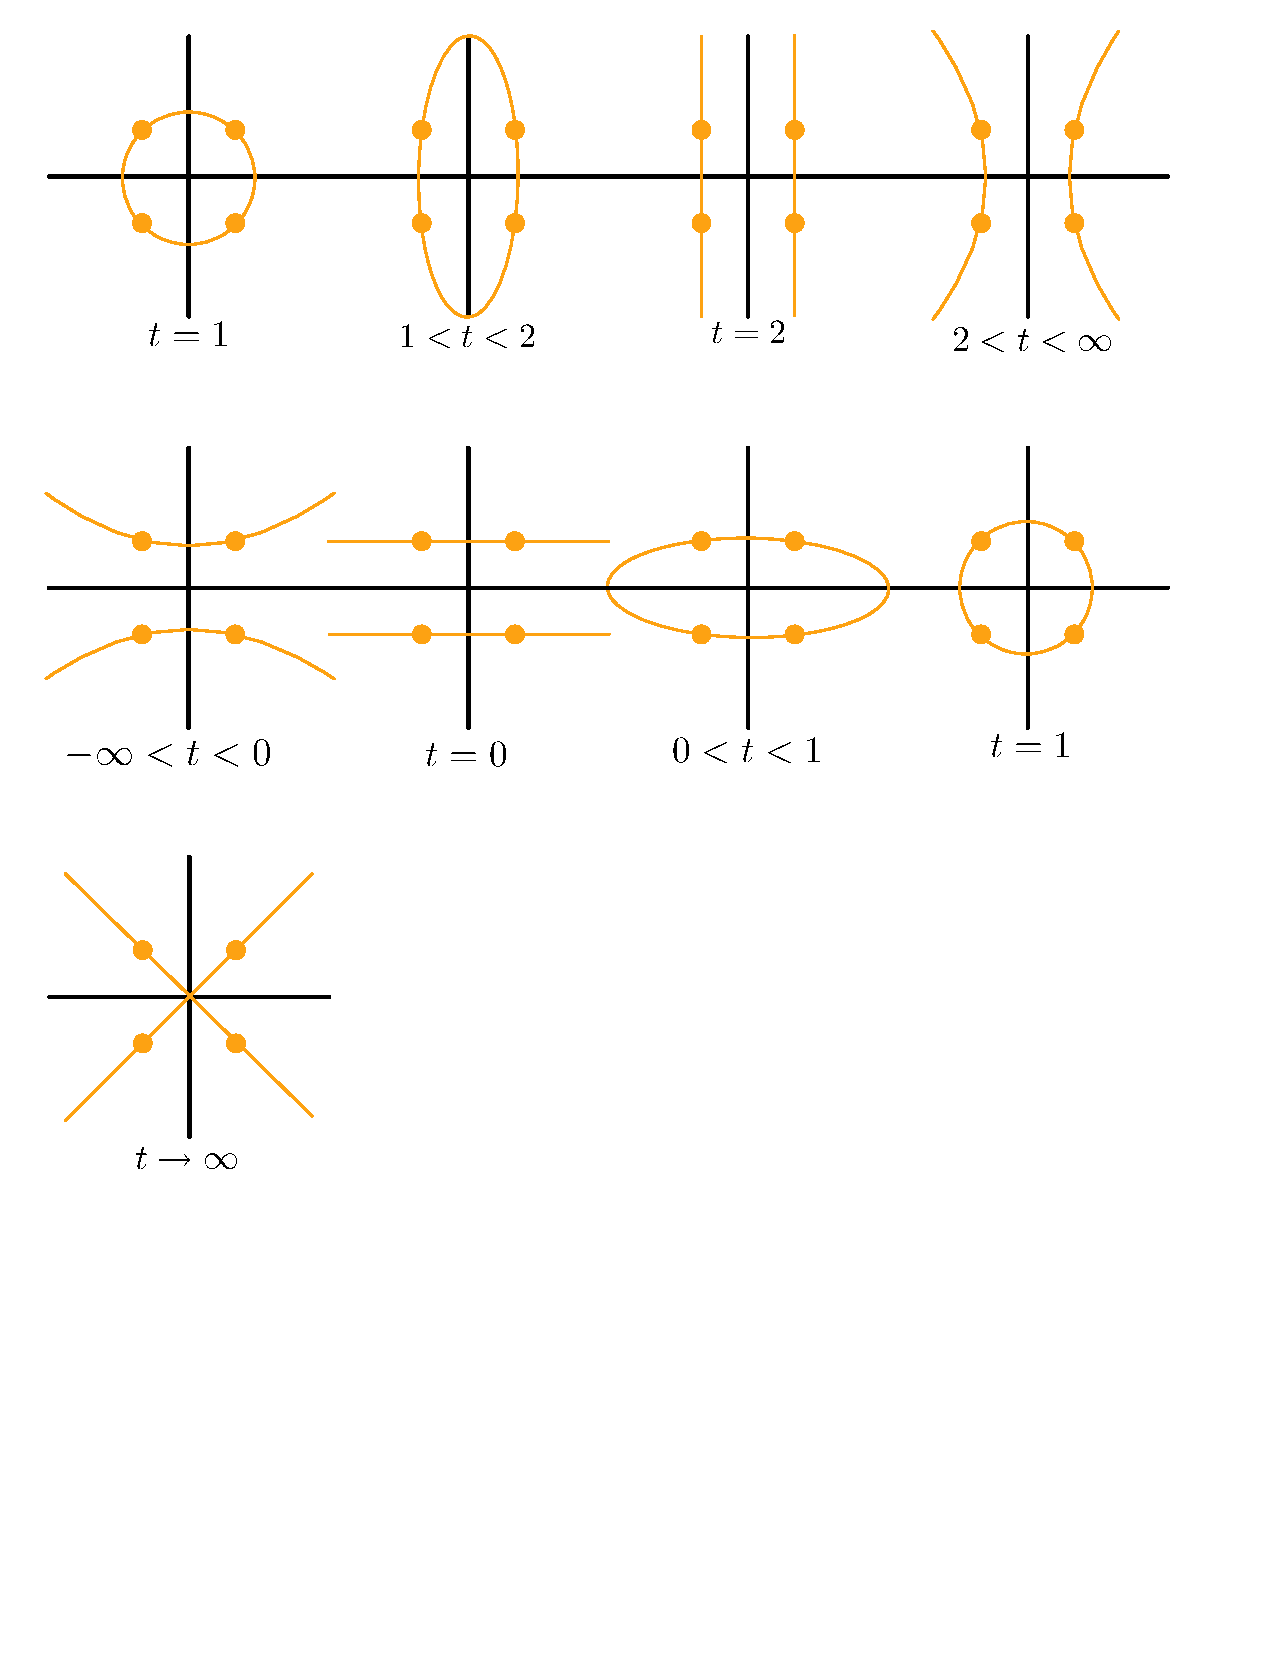
\includegraphics[width=0.3\textwidth, trim= 0.8cm 22.9cm 16cm 0.6cm,clip]{Figs/fig1Intro.pdf}
        \label{fig1Intro}
        \caption{One of the quadratic curves passing through our points: $x^2+y^2=2$.}
    \end{figure}\newpage
    Ideally we would like to stretch and shrink the circle in order to make it an ellipse. We know ellipses have equations of the form 
    $$\left(\frac xa\right)^2+\left(\frac yb\right)^2=1,$$ 
    but in order to use our circle equation we will instead add coefficients to the equation in the following fashion
    $$Ax^2+By^2=2.$$
    These coefficients are determined by the points on the curve, we may derive the relation by plugging in the coordinates of a point into the equation:
    $$A(1)^2+B(1)^2=2\To B=2-A\To tx^2+(2-t)y^2=2$$
    where we take $t=A$ to get the last equation.
    The following curves are the ones we obtain given different values of $t$:
    \vspace{-0.5em}
    \begin{itemize}
        \begin{multicols}{2}
            \itemsep=-0.4em
        \item $(t=1)$: A circle.
        \item $(1<t<2)$: An ellipse.
        \item $(t=2)$: The pair of lines $x^2=1$.
        \item $(t>2)$: A hyperbola.
        \end{multicols}
    \end{itemize}
    However we are left with one curve which passes through the points in question. To find it we will assume $t$ is non-zero. From our parametric equation we obtain 
    $$tx^2+(2-t)y^2=2\To x^2+o(t)+y^2=\frac{2}{t}\xrightarrow[t\to\infty]{}x^2=y^2$$
    which is the pair of lines $y=\pm x$. Observe that this behavior is independent of the sign of the infinity we are going to. 
    \begin{figure}[h!]
        \centering
        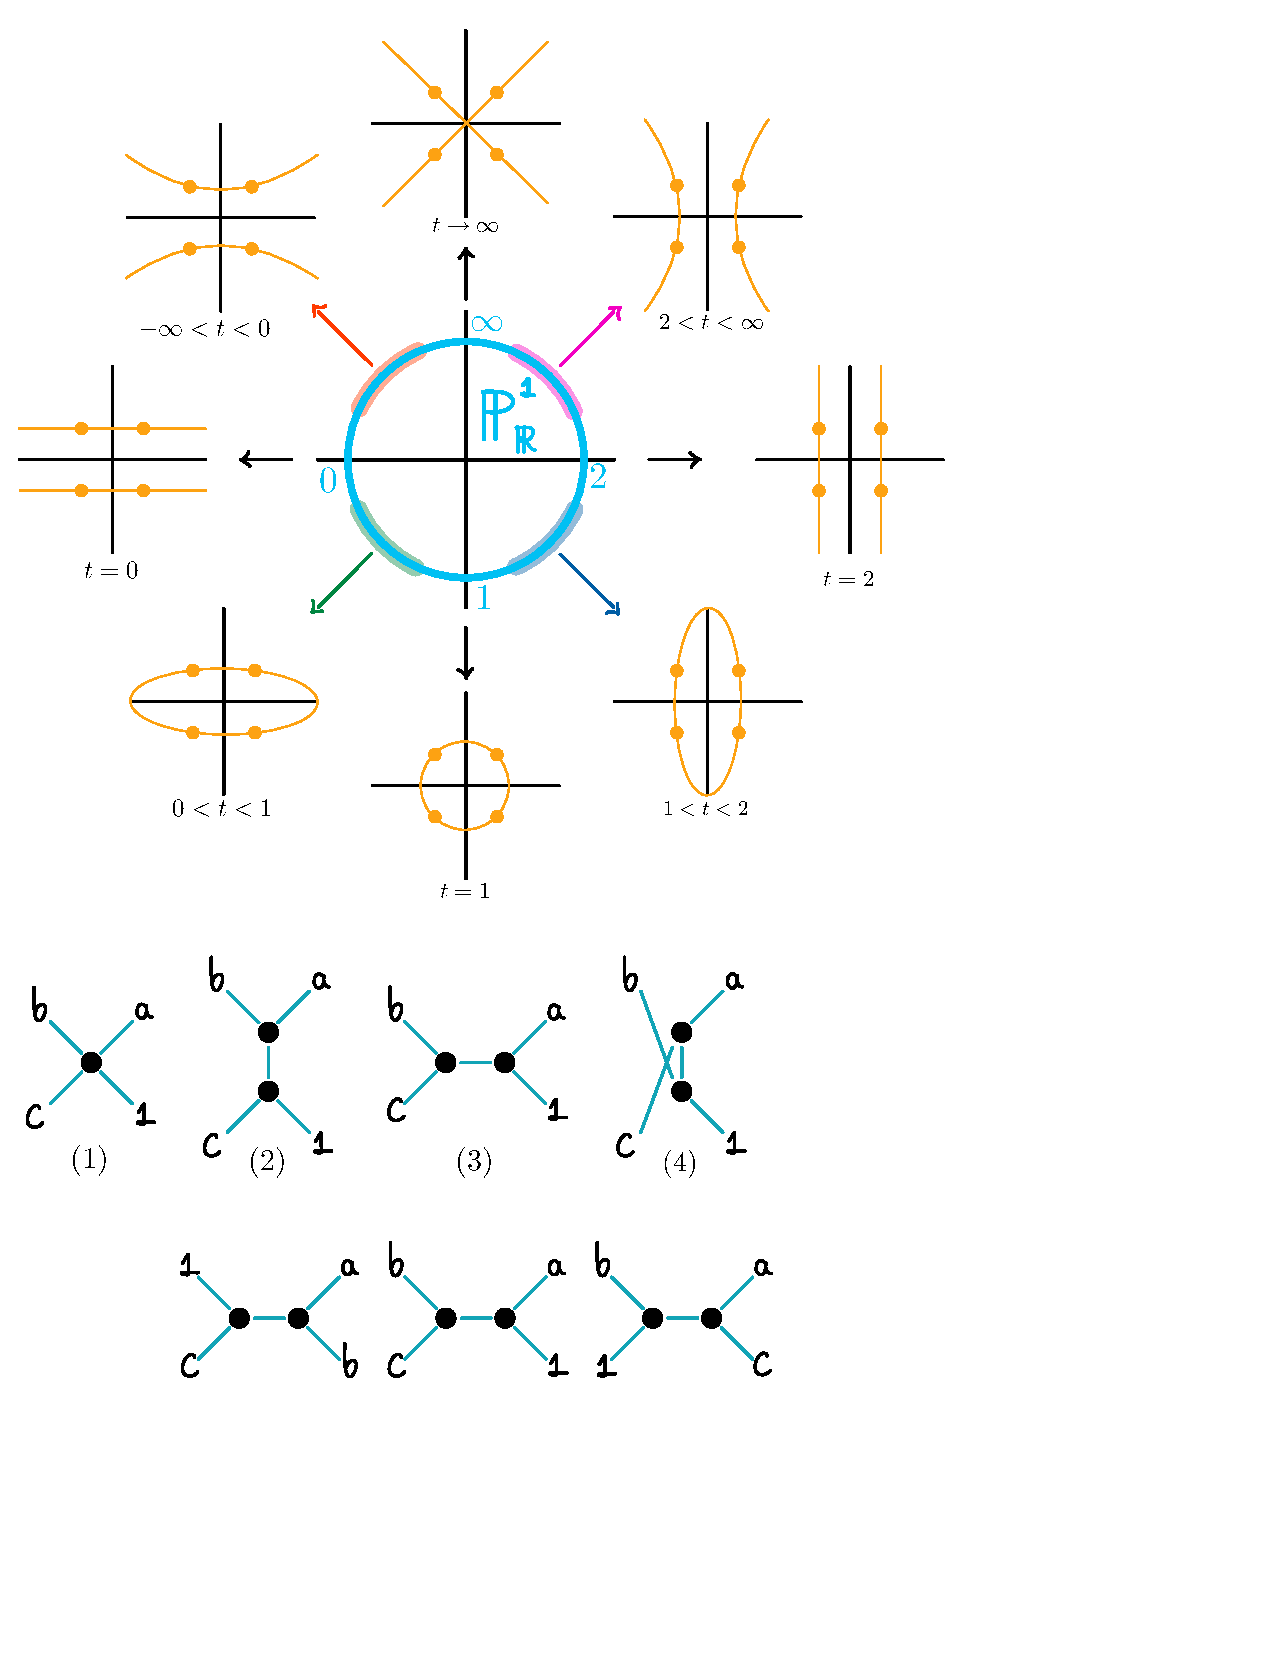
\includegraphics[width=0.8\textwidth, trim= 0.25cm 13.1cm 5.25cm 0.5cm,clip]{Figs/fig2Intro.pdf}
        \label{fig2intro}
        \caption{The projective line seen as the moduli space $\ov M_{0,4}$.}
    \end{figure}
    As such, these are all the conics passing through this four points. We omit the complex case in this example but this can be done in full generality.
\end{Ex}
   
    \iffalse
    In essence what we have seen is that all the quadratic curves passing through our set of points can be parametrized by $\bR\cup\set{\infty}$. Formally:
    \begin{Prop}\label{prop:cM04barIsomP1}
    The moduli space $\ov{\cM}_{0,4}$ can be identified with $\bP^1_\bR$.
    \end{Prop}
    Intuitively the moduli space is a set of parameters. When the points vary \emph{continuously}, the objects they parametrize deform \emph{continuously} as well. What we have done here is not a proof of the previous proposition but it may serve as evidence that it is true.\par 
    To study this space and other spaces which may arise in this fashion, we may ask a question like \emph{how many such curves can we find?} In order to do this, we will address this problem by connecting it with graphs. 
    \fi
    \newpage
This example suggests a strategy for solving the original problem for any choice of four points.

\begin{Ex}
    Given four distinct points $A$, $B$, $C$, and $D$ in general position, we look for all the possible conics passing through them.\par
    Define $F$ to be the reducible conic formed by the union of the lines through $A$ and $B$, and $C$ and $D$. Similarly, let $G$ be the conic formed by the lines through $A$ and $C$, and $B$ and $D$. Then the family of conics
    $$\la F+\mu G=0,\quad [\la,\mu]\in\bP^1$$
    describes all conics passing through the four given points.
\end{Ex}



In other words, the space of conics passing through four points in general position is naturally parametrized by $\mathbb{P}^1$. This is an example of a moduli space: a geometric space whose points parametrize certain types of objects. 

\section{A different viewpoint on the same problem}

Kapranov \cite{KapranovPaper} studied spaces which parametrized curves of certain degree passing through a number of points. The problem of classifying conics with marked points is one of such cases, and this transforms into the problem of classifying four-pointed copies of $\bP^1$. There is an equivalence between pointed curves and marked Riemann surfaces. Following this, we will emphasize the viewpoint of marked Riemann surfaces, as it better aligns with the study I have realized. 

\begin{Prop}%%%ADD FIG HERE
    \red{Fig?}Any smooth conic in the projective plane is isomorphic to the projective line.
\end{Prop}

For our four pointed conic, we get an isomorphic $(\bP^1,p_1,\dots,p_4)$. 

\begin{ptcb}
    The idea of the proof consists in taking a point in the conic from which we project lines and then create a bijection between this lines and $\bP^1$.\par
    As the conic is smooth, such lines will only have one other point of intersection with the curve meaning that we can find a bijection between points in the conic and points in the projective line.
\end{ptcb}

\begin{Rmk}
Observe that for any given four points, we will recover $\bP^1$ along different tuples of points. When we start varying the points through which the conics pass, we will obtain a different tuple. Our question is then, how do we classify this projective lines along with their points?
\end{Rmk}

\begin{Th}
    The automorphism group of $\bP^1$ is the group of Möbius transformations, $\PGL_2$. Given any two ordered triple of points 
    $$p_1,p_2,p_3\word{and}q_1,q_2,q_3$$
of the projective line, there exists a unique automorphism $T$
 of the projective line such that $T(p_i)=q_i$.
\end{Th}

We will assume the first part of this result and quickly we mention the proof for the second part.

\begin{ptcbp}
Any such automorphism is of the form 
$$z\mapsto \frac{az+b}{cz+d}$$
so let us build a map which takes $p_1,p_2,p_3$ to $0,1,\infty$ (in affine coordinates). Such a map is 
$$z\mapsto\frac{z-p_1}{z-p_3}\left(\frac{p_2-p_3}{p_2-p_1}\right).$$
    This maps $p_1,p_2,p_3$ to $0,1,\infty$ respectively. Call this map $T_p$ and then create a similar $T_q$, the desired function $T$ is $T_q^{-1}T_p$.
\end{ptcbp}

\begin{Def}
    Call the image of the fourth point $p_4$ under the aforementioned map $T_p$, the \term{cross-ratio} of the tuple $(p_1,\dots,p_4)$. 
\end{Def}

For our intents and purposes, the problem changed from
\begin{significant}
    When are two conics passing through 4 points in general position isomorphic?
\end{significant}
to the projective variant 
\begin{significant}
    When are two 4-marked projective lines isomorphic?
\end{significant}
And with the previous result we can give the answer. 

\begin{Th}
    The isomorphism class of $(\bP^1,0,1,\infty,t)$ is determined by the value $t\in\bP^1\less\set{0,1,\infty}$. 
\end{Th}

 Each smooth conic then corresponds to a $(\bP^1, 0, 1, \infty, t)$ where $t$ varies in $\bP^1 \less \set{0,1,\infty}$. Intuitively for now we will call it the moduli space of $4$-pointed $\bP^1$'s, $M_{0,4}$.\par

 But observe we are missing two things, only one of which we have talked about before. The new missing aspect is the lack of compactness of this space. $\bP^1$ as a whole is compact, but removing three points also removes that property.\par
 The other missing objects are the \emph{singular} conics. Asking where they went is like asking ``what if we let $t$ go to any of the three special points?'' We will defer the interested reader to Kock and Vainsencher's \emph{Green Book} \cite{GreenBookKockVainsencher} to fill out the details of the universal family business. In our treatment it suffices to know that whenever two points collide, we will blowup $\bP^1$ at that point adding an exceptional divisor isomorphic to $\bP^1$ and then adding the two marked points there.\par
 This treatment guarantees that $\ov M_{0,4}$ is now compact and so we have a nicer moduli space. Let us now delve deeper into this notion and throughly explain how we added the singular conics.

%%%%Aquí iba el family business

\section{Moduli of curves}

As a quick refresher, let us clarify the objects which are parametrized by the moduli spaces of our interest. 

\begin{Def}
    A \term{Riemann surface} is a complex analytic manifold of dimension $1$. 
\end{Def}

For every point in the surface, there's a neighborhood which is isomorphic to $\bC$ and transition functions are linear isomorphisms of $\bC$. We will interchangeably say Riemann surface or \emph{smooth compact complex curve}.
    
\begin{Ex}
        The following classes define Riemann surfaces.
        \begin{enumerate}
        \item $\bC$ itself is a Riemann surface with one chart.
        \item Any open set of $\bC$ is a Riemann surface.
        \item A holomorphic function $f\: U\subseteq\bC\to\bC$ defines a Riemann surface by considering $\Ga_f\subseteq\bC^2$. There's only one chart determined by the projection and the inclusion $i_{\Ga_f}$ is its inverse.
        \item Take another holomorphic function $f$, then $\set{f(x,y)=0}$ is a Riemann surface such that 
        $$\text{Sing}(f)=\set{\del_xf=\del_yf=f=0}=\emptyset.$$
        This means that at every point the gradient identifies a normal direction to the level set $f=0$. In particular, there's a well defined tangent line. The inverse function theorem guarantees that this is a complex manifold. 
        \item The first compact example is $\bP^1$.
        \end{enumerate}
\end{Ex} 

\begin{Def}
    The \term{moduli space} $M_{g,n}$ is the set of isomorphism classes of genus $g$, $n$-pointed Riemann surfaces.
\end{Def}

Recalling our motivating example, we called the space which classified the conics $M_{0,4}$. According to this definition, we are classifying $4$-pointed genus 0 Riemann surfaces. It is indeed the case that $\bP^1$ is the unique up-to-isomorphism Riemann surface of genus 0. Let us explore what happens in further genus higher up.

\begin{Ex}
    The space $M_{1,1}$ parametrizes $1$-pointed genus $1$ Riemann surfaces, or 1-marked \emph{elliptic curves}.\par
    Any such curve is isomorphic to 
    $$\quot{\bC}{L},\quad L=\bZ u+\bZ v,\word{where}u,v\in\bZ,$$
    and the image of the origin under the quotient map is the natural choice for the marked point. We have that two lattices $L_1,L_2$ determine the same elliptic curve whenever 
    $$\exists \al\in\bC^\x(L_2=\al L_1).$$
    So that 
    $$M_{1,1}=\quot{\set{\text{lattices}}}{\bC^\x}$$
    but we can be more precise!\par
    Explicitly, a lattice $L=\gen_\bZ(u,v)$ can be rescaled to
    $$\tilde{L}=\frac{1}{u}L=\gen_\bZ(1,\tau).$$
    This quantity $\tau$ always lies in the upper half plane when 
    $$\arg(v)>\arg(u)\bmod[-\pi,\pi]$$
    which means that $\tau\in\bH$ parametrizes $\bonj{\quot{\bC}{L}}$. 
    Let us apply two $\rSL_2(\bZ)=\gen(S,T)$ actions on $\tau$ which will leave the quotient unchanged:
    $$
    \left\lbrace
    \begin{aligned}
        &T\:\tau\mapsto\tau+1=\twobytwo{1}{1}{0}{1}\circ\tau=\frac{\tau+1}{0+1},\\
        &S\:\tau\mapsto-\frac1\tau=\twobytwo{0}{-1}{1}{0}\circ\tau=\frac{0-1}{\tau+0}.
    \end{aligned}
    \right.
    $$
    Then observe that the lattices
    $$\gen_\bZ(1,T\.\tau)\word{and}\gen_\bZ(1,S\.\tau)$$
    give us the same quotient. From this we can be more specific and say \red{Fig?}
    $$M_{1,1}=\quot{\bH}{\rSL_2(\bZ)}.$$
\end{Ex}

Once again, we arrive at the same issue that this space is not compact. Last time we found a way to compactify the space by adding some \emph{evidently} missing points. But it is unclear here how to deal with this conundrum. We address the problem by introducing the notion of stability.

\subsection{Stable curves}

\begin{Def}[\cite{ZvonkineIntro}, pg. 16]
    A genus $g$, $n$-pointed \term{stable curve} $(C,p_1,\dots,p_n)$ is a compact complex algebraic curve satisfying:
    \begin{enumerate}
        \item The only singularities of $C$ are simple nodes.
        \item Marked points and nodes are all distinct. Marked points and nodes do not coincide.
        \item\label{fin-number-auts} $(C,p_1,\dots,p_n)$ has a finite number of automorphisms.
    \end{enumerate}
    Throughout, we assume that stable curves are connected. The \emph{genus} of $C$ is the arithmetic genus, or equivalently, the genus of the curve obtained when \emph{smoothing the nodes}.
\end{Def}

\begin{Rmk}
Observe that the definition calls the object an \emph{algebraic curve} and not a manifold. It's almost a manifold, but it's not because it can lack smoothness.
\end{Rmk}

\begin{Th}[\cite{ZvonkineIntro}, pg. 17]
A stable curve admits a finite number of automorphisms (as in condition \ref{fin-number-auts}) if and only if every connected component $C_i$ of its normalization with genus $g_i$ and $n_i$ \emph{special} points satisfies 
$$2-2g_i-n_i<0.$$
\end{Th}

\begin{Rmk} %%%Add figure of normalization
    %https://en.wikipedia.org/wiki/Zariski%27s_main_theorem
    %https://mathoverflow.net/questions/109395/is-there-a-geometric-intuition-underlying-the-notion-of-normal-varieties
    %https://en.wikipedia.org/wiki/Normal_scheme
\red{Fig?}Normalization can be intuitively understood as the process of ``ungluing'' a variety at its singularities.\par
Formally, the normalization of a variety $X$ is a non-singular (possibly disconnected) variety $\widetilde X$ equipped with a finite birational morphism 
$$\nu:\widetilde X\to X.$$
This map is an isomorphism over the smooth locus of $X$ but may identify several points in $\widetilde X$ over a singular point of $X$. Thus, we may think of $\widetilde X$ as a version of $X$ in which the undue gluings of subvarieties. In the case of curves, normalization replaces each node with two distinct smooth points, resulting in a smooth curve (or collection of curves) marked by the preimages of the nodes. 
\end{Rmk}

\begin{ptcb}
    We will show that whenever the inequality holds, we have the components of the curve have finitely many automorphisms.\par
    Starting by considering the $g=0$ case, we may see that whenever $n\geq 3$ we have $\bP^1$'s with at least 3 marks. Thus there's no automorphisms besides the identity as any such map should fix three points.\par
    For the case of $g=1$, the inequality holds when $n$ is at least 1 as well. \red{DISCUSS Elliptic involution?}\par
    And finally for $g>2$, look at \href{https://math.stackexchange.com/questions/1680144/automorphism-group-of-genus-2-curve}{mse/1680144}
    \red{Consider hyperelliptic involution}.
    These three conditions are summarized in the inequality $2-2g_i-n_i<0$.
\end{ptcb}
\begin{Ex}
    Observe that following our motivational example, we get to the three stable curves in $\ov M_{0,4}$. Each one of these is a nodal curve where the marks and the node differ. And applying the theorem, we see that each component of the normalization satisfies
    $$2-0-3=-1<0$$
    so that we do have the stability condition. 
\end{Ex}

\begin{Ex}
    For the case of $M_{1,1}$, we compactify by adding a point representing singular stable curve. This is a one-point $\bP^1$ where we attach two points together. The resulting curve has arithmetic genus one. It can be also imagined as ``pinching a loop around the torus which doesn't go around the hole''. This is once again a stable curve as we have the stability condition:
    $$2-2(1)-1=-1<0.$$
\end{Ex}

Once equipped with the idea of stability we can now calmly talk about $\ov M_{g,n}$ as the set of isomorphism classes of \emph{stable curves}. This space can be treated as an orbifold \cite{ZvonkineIntro}, as a Deligne-Mumford stack, but we will not deal with such intricacies here. Instead, we will now delve into the cohomology of this space and talk about the combinatorial tools that will help us further along the road.

\section{Cohomological classes of the moduli space}

\subsection{The Chow ring}
%Thanks to Richard E. Borcherds here
Intuitively, for a non-singular variety $V$, we define the \emph{Chow ring} $A^\ast(V)$, whose elements \emph{correspond} to subvarieties of $V$, and the product reflects the intersection of these subvarieties. The ring is graded by codimension:
$$A^\ast(V) = \bigoplus_i A^i(V)$$
where $A^i(V)$ consists of classes of subvarieties with codimension $i$. Ideally, the intersection of a codimension $m$ subvariety $X$ and a codimension $n$ subvariety $Y$ would yield a subvariety of codimension $m+n$.\par
However, this does not always hold. Imagine a hyperplane $H$ intersected with itself. So there's a complication in defining this product.

\begin{Def}
    The $i$-th \term{Chow group} $A^i(V)$ of a non-singular variety $V$ consists of equivalence classes of codimension $i$ cycles, where two cycles are equivalent if their difference is a principal divisor, i.e., the zero set of a rational function.
\end{Def}

The \term{Chow ring} is the direct sum over all Chow groups:
$$A^\ast(V) = \bigoplus_i A^i(V)$$
The intersection product on the Chow ring is well-defined:
$$[X] \cap [Y] = \sum_{[Z]} i(X, Y; Z) [Z]$$
where $[X]$, $[Y]$, $[Z]$ denote rational equivalence classes of cycles, and $i(X, Y; Z)$ is an \emph{intersection number}, representing the multiplicity of the intersection at $Z$.

\begin{Rmk}
In the cases when we do have a transversal intersection between $X$ and $Y$, it holds that 

$$
\left\lbrace
\begin{aligned}
&[X]\cap[Y]=[X\cap Y],\\
&\codim(X\cap Y)=\codim(X)+\codim(Y).
\end{aligned}
\right.
$$

\end{Rmk}

\begin{Rmk}
    The Chow ring is related to the cohomology ring via a homeomorphism 
    $$A^i(V)\to H_{2n-2i}(V)\to H^{2i}(V)$$
    where the first map is is the cycle map, and then we apply Poincaré duality. Further exploration of the question as to where the Chow group lies inside the cohomology leads to the Hodge conjecture.
\end{Rmk}

Given the previous, we will indistinguishably call subvarieties \emph{cohomology classes of their respective codimension}. Only the basic idea of what the Chow ring as a set of isomorphism classes of subvarieties is and the idea that intersection of subvarieties corresponds to the product inside the Chow ring is essential.

\subsection{The tautological ring}

We will restrict ourselves further inside the Chow ring of $\ov M_{g,n}$. 

\begin{Def}[\cite{ZvonkineIntro}, Def. 2.6]
The minimal family of subrings $R^\ast(\ov M_{g,n})\subseteq A^\ast(\ov M_{g,n})$ stable under pushforwards by forgetful and gluing maps is called the family of \term{tautological rings} of the moduli space of stable curves.
\end{Def}

\red{
What is the meaning of a family of subrings? I thought that the tautological ring was only one. What does it mean for a family, or even just one ring, to be stable under pushforwards?
}

Intuitively, the forgetting and gluing morphisms do what we expect them to do, they either ``forget'' a marked point or ``glue'' a couple of points together.  

\begin{Def}[\cite{ArbarelloCornalba}, pg. 3]
    The \term{forgetful map} is 
    $$\pi\:\ov M_{g,n+1}\to\ov M_{g,n}$$ 
    and it assigns to a curve $(C,p_1,\dots,p_{n+1})$ the \emph{stabilization} of the curve $(C,p_1,\dots,p_n)$. Whereas the \term{gluing map} comes in two flavors. A self-gluing 
    $$\xi\:\ov M_{g-1,n+2}\to\ov M_{g,n}$$
    which takes the $(C,p_1,\dots,p_{n+1},p_{n+2})$ into $(C,p_1,\dots,p_n)$ that has a node in the place where it identified $p_{n+1},p_{n+2}$. This adds to the curve one arithmetic genus.\par
    On the other hand, the map 
    $$\eta\:\ov M_{g_1,n_1+1}\x\ov M_{g_2,n_2+1}\x\to\ov M_{g_1+g_2,n_1+n_2}$$
    glues two curves $(C_k,p_1,\dots,p_{n_k+1})$ at the points $p_{n_1+1},p_{n_2+1}$ creating a nodal curve.
\end{Def}

Intuitively, stabilization occurs when we have a $\bP^1$ component of our curve with less than 3 special points.

\begin{Ex}
    In the setting when we have a $\bP^1$-tail with 2 marks and we forget one of them, the $\bP^1$ contracts into the larger component and the mark becomes the node which just disappeared.
\end{Ex}

\red{ADD GRAPHIC Examples}
\begin{Rmk}
    One could think that an attached elliptic curve should get contracted as they have no visible marks, but they do have a special point, the node! It is in the case of pseudo-stable curves that we cannot have elliptic tails.
\end{Rmk}

Further information on stabilization can be found in \cite{GreenBookKockVainsencher} section 1.3 p. 23. But as long as we have the intuitive idea that components get contracted, we're good to go.

\subsection{Codimension 1 and combinatorial tools}

Inside the Chow ring we have the first Chow group which consists of codimension one subvarieties. 

\begin{Def}
    The boundary of the moduli space $\del M_{g,n}$ consists of all 
\end{Def}
\begin{enumerate}
    \item Talk about divisors in Mgn, what is a boundary divisor and dual trees. Para dual graphs, tesis Matt usar Arbarello Cornalba para hablar de delta a A y delta irr.
    \item $\psi$, $\la$ classes
    \item Intersection product Examples ver seccion 2.3 Matt tesis
    \item Projection formula
    \item String and Dilaton relations
    \item Integral examples
\end{enumerate}

\section{Moduli space of maps}

\chapter{Equivariant Cohomology and Localization}

\textbf{TODO}
\begin{enumerate}
    \item Basics of equivariant cohomology
 \begin{enumerate}
    \item Borel Construction of Equivariant Cohomology
    \item Examples of point equivariant Cohomology
    \item Equivariant Cohomology of projective space
\end{enumerate}
\item Localization
\begin{enumerate}
    \item Example of $H^\ast_T(\bP^r)$ through Localization
    \item Toric varieties Euler characteristic via Atiyah-Bott
    \item Hodge integral $\int_{\ov M_{0,2}(\bP^2,1)}\ev_1^\ast([1:0:0])\ev_2^\ast([0:1:0])$ via localization.
\end{enumerate}
\end{enumerate}


\section{Introduction to equivariant cohomology}

Manifolds usually don't come by themselves, like in the case of homogenous spaces, some manifolds have a lot of symmetries. These can be expressed by a group action on the manifold. We would like a cohomology theory which retains information on the group action!

\begin{Ex}[A na\"ive approach]
    Consider the $S^1$ action $\bCP^1$ given by $u\. z=uz$. This action has two fixed points, $0$ and $\infty$. Observe also that 
    $$u\.z=z\iff u=1.$$
    If we were to define the a cohomology which retains information on the group action (equivariant cohomology), we could say 
    $$H_{S^1}^\ast(\bCP^1)\defeq H^\ast(\quot{\bCP^1}{S^1}).$$
    However the orbit space $\quot{\bCP^1}{S^1}$ is the same as a closed interval which means it has trivial cohomology.
\end{Ex}

Instead of considering the cohomology of the orbit space $M/G$, which doesn't retain information on the group action, we should look for an alternive which does.

\subsection{The Borel construction}

The main idea for this concept is that homotopy equivalent spaces have the same cohomology. Suppose $G$ acts on $M$, let us create a space $EG$, a \emph{classifying space}, with the following properties:

\begin{enumerate}
    \item The right action $EG\. G$ is free. ($\forall x(\Stab(x)=0)$)
    \item $EG$ is contractible. 
    \item There exists a unique $EG$ up to homotopy. ($EG$ satisfies a universal property in a category of $G$-spaces)
\end{enumerate}

This sounds a bit risky to ask, because questions may arise. But let's avoid them for now, instead observe that 
$$M\x EG\isom M$$
as $EG$ is contractible! 

\begin{Def}
    We call the \term{orbit space}\footnote{This is now overloading the previous definition of orbit space $M/G$.} of $M$ the quotient
    $$M_G\defeq\quot{M\x EG}{(g\.x,y)\sim(x,y\.g)}.$$
    From this we define the \term{equivariant cohomology} of $M$ as 
    $$H_G^\ast(M)\defeq H^\ast(M_G).$$
\end{Def}

\begin{Ex}[Cohomology of a point]
We know that the usual cohomology of a point is trivial, but let's check two examples to see what changes.
\begin{enumerate}
    \item First consider the (trivial) action of $\bZ$ on a point. In this case we have
    $$E\bZ=\bR\word{with}x\.n=x+n.$$
    This is a free action and $\bR$ is contractible\footnote{You'll have to trust me on the fact that $\bR$ is unique up to homotopy on this one.}. Find the classifying space isn't very bad:
    $$\pt_\bZ=\quot{\bR}{x\sim x+n}\isom S^1$$
    so that 
    $$H_\bZ^\ast(\pt)=H^\ast(S^1)=\quot{\bZ[t]}{t^2}.$$
    \item Now let's take a bigger group, say $U(1)$, but for our purposes let's call it $T$ as in torus. The classifying space here is 
    $$ET=\bC^\infty\less\set{0},\word{with}\al\.\un{z}=(\al z_i)_i.$$
    The action takes a sequence of complex numbers and scalar-multiplies it by $\al\in T$. 
    %%https://mathoverflow.net/questions/198/how-do-you-show-that-s-infty-is-contractible
    This action is free, and we may see that $\bC^\infty\less\set{0}\isom S^\infty$. The infinite sphere is contractible by arguments out of my scope. And certainly, this classifying space is unique. But now, the quotient in question is 
    $$\pt_T=\quot{\bC^\infty\less\set{0}}{\un{z}\sim \al\un{z}}\isom\bP^\infty.$$
    The cohomology now is 
    $$H^\ast_{T}\pt=H^\ast\bP^\infty=\bC[t].$$
    From this example we can extend the calculation to see that for an $n$-dimensional torus $T^n$ we have 
    $$H^\ast_{T^n}\pt=H^\ast(\bP^\infty)^n=\bC[t_1,\dots,t_n]$$
    by the K\"unneth formula.
\end{enumerate}
\end{Ex}

Questions remain for me such as\dots

\begin{Qn}
    What happens when $G$ is a symmetric group $S_n$, or a finite group $\bZ/n\bZ$? Even more, what if $G$ is a matrix group, or an exceptional group such as the Mathieu group\footnote{At the time of writing, Ignacio hasn't read Classifying Spaces of Sporadic Groups by Benson and Smith.}?  
\end{Qn}

\begin{Rmk}
    One can see that the idea of constructing the cohomology of the orbit space goes haywire as soon as our space is not a point. For $\bP^1$ one has to find
    $$H^\ast\left(\quot{T^2\x\bP^2}{\sim}\right)$$
    which becomes unsurmountably hard.
\end{Rmk}

To solve this issue we ask for help with the\dots

\section{Atiyah-Bott localization theorem}

\begin{Th}[Atiyah and Bott, 1984]
    If $G\.M$ is an action and $F_k\subseteq M$ are the fixed loci of the action $G\.F_k=F_k$, then there exists an isomorphism of cohomologies
    $$H^\ast_G(M)\isom \bigoplus_kH^\ast_G(F_k)$$
    where the inclusion maps $i_k\: F_k\into M$ induce the morphisms:
    $$\un{i}^\ast\:H^\ast_G(M)\to\bigoplus_kH^\ast_G(F_k),$$
    component-wise this is the pullback of each $i_k$. And on the other direction it's
 $$\frac{i_\ast}{e(N_{\.\mid M})}\:\oplus H^\ast_G(F_k)\to H^\ast_G(M),$$ 
 where $N_{Y\mid X}$ is the normal bundle $Y\subseteq X$.
\end{Th}

To say that we're using a localization technique to find cohomology is to apply the Atiyah-Bott theorem.

\begin{Ex}[Projective line cohomology via localization]
First, let's clearly define the action of $T^2=(\bC\less\set{0})^2$ on $\bP^1$. For $\un{\al}\in T^2$ and $[X,Y]\in\bP^1$ we have
$$\un{\al}\.[X,Y]\defeq \bonj{\frac{X}{\al_1},\frac{Y}{\al_2}}\footnote{I know this is an unorthodox choice, but it's so that the weights of a certain representation are aligned properly. I'm already traumatized enough to do it the other way around.}.$$
Then, the only fixed points of this action are $0=[0:1]$ and $\infty=[1:0]$:
$$\un{\al}\.[0:1]=\bonj{0:\frac{1}{\al_2}}=[0:1],\word{and}\un{\al}\.[1:0]=\bonj{\frac{1}{\al_1}:0}=[1:0].$$
Proving that there's no more fixed points amounts to a linear algebra exercise. Applying Atiyah-Bott we now have that 
\begin{gather*}
    H_{T^2}^\ast(\bP^1)\isom H_{T^2}^\ast([0:1])\oplus H_{T^2}^\ast([1:0])\\
    \To\quot{\bC[t_1,t_2,H]}{(H-t_1)(H-t_2)}\isom \bC[t_1,t_2]\oplus\bC[t_1,t_2].
\end{gather*}
Here, we have used a calculation-not-shown which shows what the equivariant cohomology of $\bP^2$ is. But the question is, how does this isomorphism work? It suffices to see where the generators go. On the left, we have the generators $t_1, t_2$ and $H$ representing two hyperplane classes in each copy of $\bP^\infty$ and $H$ which represents the hyperplane class of $\bP^1$ as a bundle over a point. Mapping these classes we get
$$\un i^\ast\left\lbrace
\begin{aligned}
    &t_1\mapsto (t_1,t_1),\\
    &t_2\mapsto (t_2,t_2),\\
    &H\mapsto (t_1,t_2).
\end{aligned}
\right.$$
Whereas the generators on the right are the classes of the points $[0]=(1,0)$ and $[\infty]=(0,1)$. These points are mapped to the following classes:
$$i_\ast\left\lbrace
\begin{aligned}
    &[0:1]\mapsto H-t_2,\\
    &[1:0]\mapsto H-t_1.
\end{aligned}
\right.$$
And now, we are left with finding the normal bundles $N_{\pt\mid\bP^1}$. Observe that we may use the tangent-normal sequence for subspaces as follows:
$$0\to T\pt\hookto i^\ast T\bP^1\onto N_{\pt\mid\bP^1}\defeq \quot{T\bP^1}{T\pt}\to0$$
and we have that the tangent bundle to the point is actually zero. This means that we have the isomorphism
$$i^\ast T\bP^1=T_{\pt}\bP^1\isom N_{\pt\mid\bP^1}.$$
Thus the Euler classes we are looking for are for the tangent spaces above $0$ and $\infty$. These can be found using the equivariant Euler sequence for $T\bP^1$, and so we get:
$$e(N_{\.\mid\bP^1})\left\lbrace
\begin{aligned}
    &[0:1]\mapsto t_1-t_2,\\
    &[1:0]\mapsto t_2-t_1.
\end{aligned}
\right.$$
Putting this together we may see that indeed the isomorphism works as follows:
$$\left\lbrace
\begin{aligned}
    &[0:1]\mapsto \frac{H-t_2}{t_1-t_2}\mapsto\left(\frac{t_1-t_2}{t_1-t_2},\frac{t_2-t_2}{t_1-t_2}\right)=(1,0),\\
    &[1:0]\mapsto \frac{H-t_1}{t_2-t_1}\mapsto \left(\frac{t_1-t_1}{t_2-t_1},\frac{t_2-t_1}{t_2-t_1}\right)=(0,1).
\end{aligned}
\right.$$
Recall lastly that the vector $(1,0)$ represents 
$$1\.[0:1]+0\.[1:0]$$
so it's indeed the correct cohomology class.
\end{Ex}

With this example, we verified that the localization theorem indeed provides an isomorphism between different cohomology rings. Now, we use localization to compute the Euler characteristic of a different variety.

\begin{Ex}
    Consider $\bP^1\x\bP^1$ and an action of $T^4$ via rescaling all entries as before. The fixed points under this action are 
    $$(0,0),\quad(\infty,0),\quad(0,\infty),\word{and}(\infty,\infty).$$
    Let us denote by $F_k,\ k=1,\dots,4$ the cohomology classes of the fixed points, and $i_k\:F_k\hookto\bP^1\x\bP^1$ the inclusion map.
    Via the Atiyah-Bott theorem, we have that 
    \begin{align*}
    \int_{\bP^1\x\bP^1}e(T\bP^1\x\bP^1)&=\int_{\bP^1\x\bP^1}\sum_{k=1}^{4}\frac{i_{k\ast} i^\ast_k(e(T\bP^1\x\bP^1))}{e(N_{F_k\mid\bP^1\x\bP^1})}\\
    &=\sum_{k=1}^{4}\int_{F_k}\frac{ i^\ast_k(e(T\bP^1\x\bP^1))}{e(N_{F_k\mid\bP^1\x\bP^1})}\\
    &=\sum_{k=1}^{4}\int_{F_k}\frac{ e(i^\ast_kT\bP^1\x\bP^1)}{e(N_{F_k\mid\bP^1\x\bP^1})}
    \end{align*}
    and from here we invoke the tangent-normal sequence for $F_k\subseteq\bP^1\x\bP^1$. We have that 
    $$0\to TF_k\hookto i_k^\ast T\bP^1\x\bP^1\onto N_{F_k\mid\bP^1\x\bP^1}\to0.$$
    And simplifying by recalling that the tangent bundle over a point is zero, we have 
    $$0\to0\to i_k^\ast T\bP^1\x\bP^1\xrightarrow[]{\isom} N_{F_k\mid\bP^1\x\bP^1}\to0.$$
    This means that both Euler classes cancel out and we are left with just the fundamental class. The integral of the fundamental class over its own space gives us the value of $1$ so that the whole sum is equal to $4$.\par
    This lets us conclude that $\chi(\bP^1\x\bP^1)=4$.
\end{Ex}

\begin{Rmk}
    This computation did not rely on specific coordinates of $\bP^1 \times \bP^1$, only on the existence of four torus-fixed points.\par
    We also implicitly used several properties not mentioned before:
    \begin{enumerate}
        \item Chern classes commute with pullbacks, so:
        $$i_k^\ast(e(T\bP^1\x\bP^1))=e(i_k^\ast T\bP^1\x\bP^1).$$
        \item Integration against a pushforward restricts to the domain of the map:
        $$\int_{\bP^1\x\bP^1}i_{k\ast}(\.)=\int_{F_k}$$
    \end{enumerate}
\end{Rmk}

The variety $\bP^1 \times \bP^1$ is an example of a \emph{toric variety}. One property of toric varieties is that their Euler characteristic is equal to the number of torus-fixed points.

\begin{Def}
    A \term{toric variety} is an irreducible variety $X$ containing a torus $T^k\defeq(C\less\set{0})^k$ as a Zariski open subset such that the action of $T^k$ on itself extends to a morphism $T^k\x X\to X$.
\end{Def}

In general, for toric varieties, the number of torus-fixed points equals the number of top-dimensional cones in the associated fan which is combinatorial information that can be computed easily.

\begin{Th}
For a toric variety, the Euler characteristic equals the number of torus-fixed points under the torus action.
\end{Th}

%%%%%%%%%%%% Contents end %%%%%%%%%%%%%%%%
\ifx\nextra\undefined
\printindex
\else\fi
\nocite{*}
\bibliographystyle{plain}
\bibliography{../bibiDoctoralNotebook.bib}
\end{document}